\documentclass[a4paper]{book}

% Add styles directory to search path
\makeatletter
\def\input@path{{styles/}}
\makeatother

\def\TextOrHandout{text}
%\def\TextOrHandout{handout}

\usepackage{amssymb,amsmath,amsthm,graphicx,mathrsfs}
\usepackage{fontspec}
\usepackage[utf8]{inputenc} 
\usepackage{geometry} 
\usepackage{tikz} 
\usepackage{xcolor}
\usepackage{amsrefs}
\usepackage[bookmarks]{hyperref}
\usepackage{lipsum}  
\usepackage{forloop}
\usepackage{ifthen}
\usepackage[most]{tcolorbox}
\usepackage{pygmentex}
\tcbuselibrary{minted}
%\usepackage{minted2}
\usepackage{minted}
\usepackage{setspace}
\onehalfspacing
\tcbuselibrary{theorems}
\usetikzlibrary{shapes.geometric}
\usepackage{enumitem}
\setlist[enumerate]{itemsep=0mm}

\usepackage{imakeidx}
\makeindex

\linespread{1.5} 

\setmainfont{Browallia New}[Scale=1.5]
%\fontspec{Browallia New}[Scale=3]
\XeTeXlinebreaklocale "th"

\title{คณิตศาสตร์ดีสครีตสำหรับการเขียนโปรแกรม\\(Discrete Mathematics for Programming)}
\author{Phaphontee Yamchote}
\date{}

%\newtheorem{thm}{Theorem}
%\newtheorem{prop}{Proposition}
%\newtheorem{lem}{Lemma}

\theoremstyle{definition}
\newtheorem{defin}{Definition}[section]
\newtheorem{exam}[defin]{Example}
\newtheorem{exer}[defin]{Exercise}

\newcommand{\R}{\mathbb{R}}
\newcommand{\N}{\mathbb{N}}
\newcommand{\Z}{\mathbb{Z}}
\newcommand{\Q}{\mathbb{Q}}


\newcommand{\boxrule}[2]{
		{~\newline~\newline\centering
		\begin{tikzpicture}
			\node[anchor=text,text width=\columnwidth-0.5cm, draw, rounded corners, line width=1pt, fill=gray!10, inner sep=3mm] (big) {\newline#2};
			\node[draw, rounded corners, line width=.5pt, fill=yellow!40, anchor=west, xshift=2.5mm] (small) at (big.north west) {\textbf{#1}};
		\end{tikzpicture}}
}

\newcommand{\boxnote}[2]{
	{~\newline~\newline\centering
		\begin{tikzpicture}
			\node[anchor=text,text width=\columnwidth-0.5cm, draw, rounded corners, line width=0.5pt, fill=white, inner sep=3mm] (big) {\\#2};
			\node[draw, rounded corners, line width=.5pt, fill=gray!40, anchor=west, xshift=2.5mm] (small) at (big.north west) {#1};
	\end{tikzpicture}}
}

\newcommand{\solution}[1]{
	\ifthenelse{\equal{\TextOrHandout}{handout}}{\vspace{5 cm}}{\paragraph{Solution.} #1~\newline}
}

\definecolor{bg}{rgb}{0.95,0.95,0.95}

%%%%%%%%%%%%%%%%%%%%%%%%%%%%%%%%%%%%%%%%%%%%%
%%%%%%%%%%%%%%%%%%%%%%%%%%%%%%%%%%%%%%%%%%%%%
%%										   %%%
%%             Python code				   %%%
%%										   %%%
%%%%%%%%%%%%%%%%%%%%%%%%%%%%%%%%%%%%%%%%%%%%%
%%%%%%%%%%%%%%%%%%%%%%%%%%%%%%%%%%%%%%%%%%%%%

\tcbset{
	pythoncodebox/.style={
		enhanced jigsaw,breakable,
		colback=gray!10,colframe=gray!20!black,
		boxrule=1pt,top=2pt,bottom=2pt,left=2pt,right=2pt,
		sharp corners,before skip=10pt,after skip=10pt,
		attach boxed title to top left,
		boxed title style={empty,
			top=0pt,bottom=0pt,left=2pt,right=2pt,
			interior code={\fill[fill=tcbcolframe] (frame.south west)
				--([yshift=-4pt]frame.north west)
				to[out=90,in=180] ([xshift=4pt]frame.north west)
				--([xshift=-8pt]frame.north east)
				to[out=0,in=180] ([xshift=16pt]frame.south east)
				--cycle;
			}
		},
		title={#1}, % Argument of pythoncodebox specifies the title
		fonttitle=\sffamily\bfseries
	},
	pythoncodebox/.default={}, % Default is No title
	%%% Starred version has no frame %%%
	pythoncodebox*/.style={
		enhanced jigsaw,breakable,
		colback=gray!10,coltitle=gray!20!black,colbacktitle=tcbcolback,
		frame hidden,
		top=2pt,bottom=2pt,left=2pt,right=2pt,
		sharp corners,before skip=10pt,after skip=10pt,
		attach boxed title to top text left={yshift=-1mm},
		boxed title style={empty,
			top=0pt,bottom=0pt,left=2pt,right=2pt,
			interior code={\fill[fill=tcbcolback] (interior.south west)
				--([yshift=-4pt]interior.north west)
				to[out=90,in=180] ([xshift=4pt]interior.north west)
				--([xshift=-8pt]interior.north east)
				to[out=0,in=180] ([xshift=16pt]interior.south east)
				--cycle;
			}
		},
		title={#1}, % Argument of pythoncodebox specifies the title
		fonttitle=\sffamily\bfseries
	},
	pythoncodebox*/.default={}, % Default is No title
}
% Custom tcolorbox for Python code (not the code itself, just the box it appears in)
\newtcolorbox{pythonbox}[1][]{pythoncodebox=#1}
\newtcolorbox{pythonbox*}[1][]{pythoncodebox*=#1} % Starred version has no frame

% Custom minted environment for Python code, NOT using tcolorbox
\newminted{python}{autogobble,breaklines,mathescape}

% Custom tcblisting environment for Python code, using the "minted" tcb listing engine
% Adapted from https://tex.stackexchange.com/a/402096
\NewTCBListing{python}{ !O{} !D(){} !G{} }{
	listing engine=minted,
	listing only,
	pythoncodebox={#1}, % First argument specifies the title (if any)
	minted language=python,
	minted options/.expanded={
		autogobble,breaklines,mathescape,
		#2 % Second argument, delimited by (), denotes options for the minted environment
	},
	#3 % Third argument, delimited by {}, denotes options for the tcolorbox
}

%%% Starred version has no frame %%%
\NewTCBListing{python*}{ !O{} !D(){} !G{} }{
	listing engine=minted,
	listing only,
	pythoncodebox*={#1}, % First argument specifies the title (if any)
	minted language=python,
	minted options/.expanded={
		autogobble,breaklines,mathescape,
		#2 % Second argument, delimited by (), denotes options for the minted environment
	},
	#3 % Third argument, delimited by {}, denotes options for the tcolorbox
}

% verbbox environment, for showing verbatim text next to code output (for package documentation and user learning purposes)
\NewTCBListing{verbbox}{ !O{} }{
	listing engine=minted,
	minted language=latex,
	boxrule=1pt,sidebyside,skin=bicolor,
	colback=gray!10,colbacklower=white,valign=center,
	top=2pt,bottom=2pt,left=2pt,right=2pt,
	#1
} % Last argument allows more tcolorbox options to be added
%%%%%%%%%%%%%%%%%%%%%%%%%%%%%%%%%%%%%%%%%%%%%
%%%%%%%%%%%%%%%%%%%%%%%%%%%%%%%%%%%%%%%%%%%%%
%%										   %%%
%%            end of Python code		   %%%
%%		 								   %%%
%%%%%%%%%%%%%%%%%%%%%%%%%%%%%%%%%%%%%%%%%%%%%
%%%%%%%%%%%%%%%%%%%%%%%%%%%%%%%%%%%%%%%%%%%%%

\tcbuselibrary{theorems}

\newtcbtheorem[use counter*=defin,number within=section]{defn}{นิยาม~}%
{colback=yellow!0,colframe=black,fonttitle=\bfseries,colbacktitle=white,coltitle=black}{}
%
\newtcbtheorem[use counter*=defin,number within=section]{lem}{บทตั้ง}%
{colback=yellow!0,colframe=black,fonttitle=\bfseries}{}

\newtcbtheorem[use counter*=defin,number within=section]{prop}{คุณสมบัติ}%
{colback=yellow!0,colframe=black,fonttitle=\bfseries}{}

\newtcbtheorem[use counter*=defin,number within=section]{thm}{ทฤษฎีบท}%
{colback=yellow!0,colframe=black,fonttitle=\bfseries}{}

\newcommand{\progpart}{
	\begin{center}
		\title{\sffamily\colorbox{black}{\bfseries\textcolor{white}{\Large PROGRAMMING PART}}}
	\end{center}
}

\newcommand{\theopart}{
	\begin{center}
		\title{\sffamily\colorbox{black}{\bfseries\textcolor{white}{\Large THEORY PART}}}
	\end{center}
}

\newcommand{\proofpart}{
	\begin{center}
		\title{\sffamily\colorbox{black}{\bfseries\textcolor{white}{\Large PROOF PART}}}
	\end{center}
}

\renewenvironment{proof}{~\newline~\textbf{บทพิสูจน์}.}{$\square$}

\begin{document}
	\maketitle
	\frontmatter
	\tableofcontents

	\mainmatter

    \part{Basic Programming by Python}
    \chapter{Fundamental of Problem Solving}

เราจะเริ่มบทแรกของหนังสือเล่มนี้ด้วยทักษะที่สำคัญที่สุดไม่ว่าจะในการเรียนคณิตศาสตร์ หรือจะคอมพิวเตอร์ก็ตาม นั่นคือทักษะการแก้ปัญหา (problem solving) เพราะแก่นแท้ของตัววิชาเหล่านี้นั้นคือการนำความรู้ไปใช้ในการแก้ปัญหาต่าง ๆ ไม่ว่าจะปัญหาในตัววิชาเองในรูปแบบปัญหาเชิงการคำนวณ (computational problem) หรือปัญหาในโลกจริง กล่าวคือ ปัญหาคือสิ่งที่เราจะต้องพบเจอเป็นเรื่องปกติในการเรียนวิชานี้

ในบทนี้เราจะเริ่มจากมาดูกันก่อนว่าปัญหาคืออะไร และการแก้ปัญหาคืออะไร เพราะก่อนจะลงมือแก้ปัญหา เราก็ต้องเข้าใจก่อนว่าสิ่งเหล่านี้คืออะไร หลังจากที่เข้าใจเกี่ยวกับสิ่งที่เรียกว่าปัญหาแล้ว เราจะมาต่อกันว่าทักษะหรือแนวคิดอะไรบ้างที่สำคัญในการแก้ปัญหา โดยจะไม่กล่าวถึงรายละเอียดปลีกย่อยของเทคนิคการแก้ปัญหา เพราะในแต่ละรูปแบบปัญหาที่ต่างกัน ก็จะมีรายละเอียดในเรื่องวิธีการแก้ปัญหาหรือเทคนิคการแก้ปัญหาที่แตกต่างกันออกไป เหมือนการทำโจทย์คณิตศาสตร์ที่รูปแบบโจทย์ที่แตกต่างกันก็อาจจะมีเทคนิคที่แตกต่างกัน แต่ว่าสิ่งที่จะทำให้เรารู้ว่าต้องใช้เทคนิคหรือวิธีการอะไรในการแก้ปัญหาที่ต้องการแก้ก็คือประสบการณ์ที่เราจะได้ฝึกกันในแต่ละบท ๆ ต่อจากนี้นั่นเอง

\section{Problem Solving คืออะไร}

ก่อนจะถามว่าการแก้ปัญหาคืออะไร ก็คงไม่เสียเวลาอะไรนักถ้าเราจะมาพูดคุยตกลงกันให้เข้าใจก่อนว่า อะไรคือ\textbf{ปัญหา} ซึ่งถ้าเราเปิดดูความหมายตามราชบัณฑิต คำนี้จะมีความหมายว่า
\begin{center}
	น. ข้อสงสัย, ข้อขัดข้อง, เช่น ทำได้โดยไม่มีปัญหา, คำถาม, ข้อที่ควรถาม, เช่น ตอบปัญหา, ข้อที่ต้องพิจารณาแก้ไข เช่น ปัญหาเฉพาะหน้า ปัญหาทางการเมือง.
\end{center}
ซึ่งบางความหมาย อาจจะรู้สึกว่าปัญหาก็คืออะไรที่รู้สึกว่าไม่ดี เพราะจะทำให้สิ่งต่าง ๆ ดำเนินไปไม่เป็นไปตามที่ควรจะเป็น เช่นข้อขัดข้อง หรือข้อที่ต้องพิจารณาแก้ไข ทว่ายังมีความหมายอีกกลุ่มหนึ่งที่ดูน่าสนใจคือ ข้อสงสัย ข้อควรถาม ที่เรามักพูดกันว่า ``ตอบปัญหา''

ในหนังสือเล่มนี้ (และในคณิตศาสตร์ รวมไปถึงการเขียนโปรแกรมคอมพิวเตอร์) เราจะให้ความหมายของ \textbf{ปัญหา} คือ โจทย์ที่ถามหรือกล่าวขึ้นมาพื่อต้องการคำตอบโดยอาจจะมีเงื่อนไขบางอย่างหรือไม่มีก็ได้ โดยจะเป็นการกล่าวถึงสถานการณ์ที่มีสิ่งตั้งต้นอะไรสักอย่าง แล้วสุดท้าย(หลังจากผ่านกระบวนการอะไรสักอย่าง)จะได้สิ่งที่ต้องการออกมา

ตัวอย่างเช่น ``บริษัทจัดสรรแม่บ้านทำความสะอาดตามสั่งแห่งหนึ่งได้รับการจองคิวใช้บริการแม่บ้านเข้ามาจำนวนหนึ่งจากลูกค้าหลายราย โดยที่ลูกค้าแต่ละคนก็มีจำนวนวันที่ต้องการใช้บริการแม่บ้านไม่เหมือนกัน ทางบริษัทเลยอยากรู้ว่าต้องเตรียมแม่บ้านไว้กี่คน'' ซึ่งเราจะพบว่าปัญหานี้เราต้องการรู้ว่าต้องเตรียมแม่บ้านไว้กี่คน โดยเรามีรายการการจองคิวเป็นตัวตั้งของการตอบปัญหานี้

จากตัวอย่างที่กล่าวมา จะเรียกสิ่งตั้งต้น (เช่นรายการการจองคิวที่บริษัทได้รับ) ว่า\textbf{ข้อมูลขาเข้า} (input) และเราจะเรียกสิ่งที่ได้ออกมา (เช่นจำนวนแม่บ้านที่ต้องเตรียมไว้) ว่า\textbf{ข้อมูลขาออก} (output) ดังนั้น เราอาจจะกล่าวได้อีกแบบหนึ่งว่าปัญหาก็คือการมีข้อมูลขาเข้า และข้อมูลขาออกที่ต้องการ และสิ่งที่เราต้องลงแรงหาก็คือ วิธีการที่จะแปลเปลี่ยนข้อมูลขาเข้าดังกล่าวให้ได้ข้อมูลขาออกตามที่ต้องการ ซึ่งเราจะเรียกกระบวนการการหาวิธีการดังกล่าวว่า\textbf{การแก้ปัญหา} (problem solving) และจะเห็นว่าสิ่งสำคัญอันดับแรกสุดไม่ว่าเราจะแก้ปัญหาอะไรก็ตามคือการทำความเข้าใจภาพรวมของโจทย์ (problem statement) ว่าตัวปัญหาคืออะไร และระบุให้ได้ว่าอะไรคือข้อมูลขาเข้า และข้อมูลขาออก โดยถ้าเทียบกับตัวอย่างบริษัทแม่บ้านทำความสะอาดก่อนหน้า จะมีรายละเอียดดังนี้

\begin{itemize}
	\itemsep0em 
	\item \textbf{โจทย์}: หาวิธีการในการคำนวณจำนวนแม่บ้านที่ต้องเตรียมไว้เมื่อได้รับรายการการจองคิวใช้บริการจากลูกค้า
	\item \textbf{ข้อมูลขาเข้า}: รายการการจองคิวใช้บริการ
	\item \textbf{ข้อมูลขาออก}: จำนวนแม่บ้านที่ต้องเตรียมไว้
\end{itemize}

ทั้งนี้ ตัวปัญหาเองก็อาจจะถูกแบ่งกลุ่มออกเป็นประเภทต่าง ๆ ได้หลายประเภท แต่ปัญหาที่เราจะสนใจกันในหนังสือเล่มนี้นั้นจะเป็นปัญหาในกลุ่ม\textbf{ปัญหาเชิงการคำนวณ} (computational problem) หรือหนังสือบางเล่มจะเรียกว่าปัญหาเชิงการประมวลผล ซึ่งคำว่าคำนวณในที่นี่ไม่ได้หมายถึงเพียงแค่การบวก ลบ คูณ หาร หรือการทำโจทย์คณิตศาสตร์ (calculation) แต่ยังรวมไปถึงการวางแผนเชิงกระบวนการ เชิงตรรกะ เชิงเหตุผล หรือรวมไปถึงการคิดเชิงสัญลักษณ์เองก็ด้วย ไม่จำเป็นว่าจะต้องเป็นปัญหาที่เกี่ยวกับตัวเลขเพียงเท่านั้น ซึ่งกระบวนการการแก้ปัญหาเชิงการคำนวณถือว่าเป็นทักษะที่สำคัญที่สุดในการเขียนโปรแกรม รวมไปถึงการศึกษาคณิตศาสตร์ และวิทยาการคอมพิวเตอร์ โดยเราจะได้กล่าวถึงรายละเอียดของกระบวนการดังกล่าวในหัวข้อถัดไป

\section{การแก้ปัญหาเชิงการคำนวณ}

จากหัวข้อที่แล้ว เราอาจกล่าวโดยสรุปได้ว่าปัญหาเชิงการคำนวณก็คือปัญหาที่จะสามารถแก้ได้ด้วยคอมพิวเตอร์โดยการออกแบบอัลกอริทึมที่เหมาะสม และในการแก้ปัญหาเชิงการคำนวณนั้น จะมีทักษะที่สำคัญที่จะช่วยให้เราแก้ปัญหาเชิงการคำนวณได้อย่างมีประสิทธิภาพอยู่ 4 ทักษะได้แก่
\begin{enumerate}
	\itemsep0em 
	\item การแบ่งย่อยปัญหา (decomposition)
	\item การเข้าใจรูปแบบ (pattern recognition)
	\item การคิดเชิงนามธรรม (abstraction)
	\item การออกแบบขั้นตอนวิธี (algorithm design)
\end{enumerate}

\subsection{การแบ่งย่อยปัญหา (decomposition)}
ในการแก้ปัญหาหนึ่งที่เราได้รับมานั้น อาจเป็นการยากถ้าเราจะหาวิธีที่แปลงข้อมูลขาเข้าให้กลายเป็นข้อมูลขาออกได้ภายในขั้นเดียว อาจจะเนื่องมาจากการแก้ปัญหาดังกล่าวต้องการขั้นตอนย่อย ๆ หรือเครื่องมือย่อย ๆ ในการแก้ปัญหานั้น ดังนั้นเราจึงควรย่อยปัญหาใหญ่ให้ออกเป็นปัญหาย่อย ๆ ที่จะสามารถแก้ได้ง่าย ๆ ไม่ซับซ้อนก่อน

ตัวอย่างเช่นเราอยากจะต่อจิกซอว์สักรูปหนึ่ง คงเป็นการยากถ้าเราจะเทจิกซอว์ทั้งหมดลงมาในแผ่นเดียวแล้วต่อขึ้นมาด้วยการมองภาพทั้งภาพในเวลาเดียวกัน แต่คงจะดีขึ้นถ้าเรารู้ว่าในภาพมีองค์ประกอบย่อย ๆ ที่เห็นความแตกต่างเรื่องสีอย่างชัดเจน เช่นมีบริเวณหนึ่งที่มีแต่สีแดง และมีอีกบริเวณหนึ่งที่มีแต่สีเขียว หรืออีกบริเวณหนึ่งเป็นลายผ้าสีเหลืองลายจุดสีส้ม เราก็เลยจะแบ่งปัญหาการต่อจิกซอว์ทั้งผืนเป็นปัญหาการต่อจิกซอว์กลุ่มย่อย ๆ ที่เป็นสีแดง, ปัญหาการต่อจิกซอว์กลุ่มย่อย ๆ ที่เป็นสีเขียว และ ปัญหาการต่อจิกซอว์กลุ่มย่อย ๆ ที่เป็นสีเหลืองลายจุดสีส้ม ซึ่งจะทำให้เกิดปัญหาที่เล็กลงและอาจจะซับซ้อนน้อยลงเพราะเรากำจัดตัวเลือกจิกซอว์ที่ไม่เกี่ยวข้องกับบริเวณดังกล่าวออกไปได้เยอะ

ขออีกสักตัวอย่างที่ดูเป็นปัญหาเชิงการคิดเลขมากขึ้น เช่นปัญหาการแก้สมการจำนวนเต็ม $x + y + 12z = 30$ โดยที่ $x, y$ และ $z$ เป็นจำนวนเต็มบวกสามจำนวนที่ต่างกัน โดยโจทย์ต้องการว่ามีผลเฉลย $(x,y,z)$ ดังกล่าวทั้งหมดกี่ครูปแบบ ซึ่งแน่นอนว่าถ้าเราไล่ไปเรื่อย ๆ ก็อาจจะเสร็จได้ไม่ได้ยากมาก เพราะเลขเราต้องการผลบอกแค่ 30 ถ้าต้องไล่ 0 ถึง 30 ก็มีอยู่ไม่เกิน $31 \times 31 \times 31 = 29791$ รูปแบบ ซึ่งถ้าให้คอมพิวเตอร์ช่วยรันให้ก็คงใช้เวลาไม่นาน แต่ถ้าใช้คนก็อาจจะเหนื่อยก่อนและมีคิดผิดบ้างได้ แต่เราจะเห็นว่าการเพิ่มขึ้นของค่า $z$ นั้นกลับมีประโยชน์อย่างมาก เพราะเพิ่มขึ้น 1 ค่าในด้านซ้ายจะเพิ่มขึ้นไปถึง 12 ดังนั้นเราจึงอาจจะสังเกตได้ไม่ยากว่าแยกพิจารณาตามค่า $z$ ไปเลยก็ได้ โดยที่ $z = 0,1,2$ (เพราะถ้ามากกว่านี้ ผลบวกจะเกิน 30) กล่าวคือ เราจะแยกปัญหาหลักเราออกเป็นปัญหาย่อย 3 ปํญหาย่อยคือ
\begin{enumerate}
	\itemsep0em 
	\item เมื่อ $z = 0$: แก้สมการ $x + y = 30$
	\item เมื่อ $z = 1$: แก้สมการ $x + y = 18$
	\item เมื่อ $z = 2$: แก้สมการ $x + y = 6$
\end{enumerate}
ซึ่งแต่ละปัญหาย่อย จะสามารถแก้ได้ด้วยการนับง่าย ๆ

ในการแยกปัญหาย่อยนั้น อาจจะได้ปัญหาย่อยมาในรูปแบบที่แยกกันทำ ต่างคนต่างอิสระจากกัน ทำเสร็จแล้วค่อยนำคำตอบของแต่ละปัญหามาผนวกรวมร่างกันให้กลายเป็นปัญหาใหญ่ เช่นตัวอย่างสมการข้างต้นที่เราสามารถแก้ปัญหาไหนก่อนก็ได้ไม่มีผลต่อกัน หรือเราอาจจะได้ปัญหาย่อยที่มาในรูปแบบที่ต้องทำงานต่อเนื่องกันโดยที่เมื่อทำปัญหาย่อยที่ 1 เสร็จให้นำผลของปัญหาย่อยที่ 1 ไปใช้ต่อเป็นข้อมูลขาเข้าของปัญหาย่อยที่ 2 ก็ได้ ทั้งนี้ ไม่มีกฏตายตัวในการตั้งปัญหาย่อย ขึ้นอยู่กับมุมมองต่อปัญหาตรงหน้าของเรา ณ เวลานั้น

\subsection{การเข้าใจรูปแบบ (pattern recognition)}
ใน





    \chapter{Basic Python Syntax}

%    
   	\part{Basic Mathematical Reasoning and Proving}
   	\chapter{Mathematics as a Language}\label{chap:mathLang}

บทนี้จะเป็นบทสั้น ๆ เน้นที่การเล่าให้เห็นภาพรวมของคณิตศาสตร์ในรูปแบบการเรียนเพื่อหาเหตุผล เป้าหมายของบทนี้เพียงเพื่อต้องการเปลี่ยนทัศนคติของผู้อ่านบางท่านเกี่ยวกับคณิตศาสตร์ ก่อนที่เราจะลงลึกไปสู่คณิตศาสตร์จริง ๆ ในบทถัด ๆ ไป อย่างน้อยก็อยากให้หลังจากที่อ่านบทนี้จบ ผู้อ่านจะมองว่าคณิตศาสตร์คือวิชาของการอธิบายสิ่งต่าง ๆ ในโลก และการให้เหตุผลของความเป็นไปในสิ่งต่าง ๆ ไม่ใช่แค่การคิดเลข

หลายท่าน (รวมถึงเด็ก ๆ จากประสบการณ์การสอนพิเศษมาหลายปีของผู้เขียน) อาจจะจำความรู้สึกมาจากตอนเรียนระดับมัธยมต้นว่าวิชาคณิตศาสตร์เป็นวิชาที่เกี่ยวกับการคิดเลข จำสูตรไปแทนค่าหาคำตอบ ขอแค่จำสูตรไดเ้ยอะ ๆ อ่านโจทย์แล้วรู้ว่าใช้สูตรไหน คิดเลขให้ไว ๆ ก็น่าจะทำข้อสอบได้คะแนนดีกันแล้ว ผู้เขียนเคยเจอถึงขั้นว่ามีนักเรียนใช้วิธีดูว่าข้อนี้ต้องหยิบสูตรไหนมาคิดโดยการดูว่าเจอคีย์เวิร์ดอะไรในโจทย์ และบอกคนอื่นได้ว่าเราเรียนคณิตศาสตร์รู้เรื่อง แต่ทว่า พอขึ้นมาเรียนในระดับมัธยมปลาย กลับพบว่าคณิตศาสตร์เปลี่ยนไปอย่างมาก เราได้เรียนเรื่องเซต เรื่องตรรกศาสตร์ ความสัมพันธ์และฟังก์ชันในระดับชั้นมัธยมศึกษาปีที่ 4 กันเป็นเรื่องแรก ๆ ที่ตัวเนื้อหาตามหนังสือเรียนนั้น แทบไม่ใช่การคิดเลขเลย แต่เป็นเรื่องของการเรียนรู้การใช้สัญลักษณ์ เรียนรู้การให้เหตุผล เพื่อใช้สื่อสารกันในโลกของคณิตศาสตร์ ซึ่งอาจจะต้องโทษวิธีการสอนของครูมัธยมไทยหลาย ๆ ท่านที่ทำให้เนื้อหาพวกนี้หนีไม่พ้นสอนการคิดเลขเหมือนเดิม เช่น\textbf{จัดรูป}อย่างง่ายของประพจน์ \textbf{คำนวณ}หาผลยูเนียน \textbf{คำนวณ}หาผลอินเตอร์เซคชัน หรือแม้กระทั่ง\textbf{คำนวณ}หาผลค่าความจริงในวิชาตรรกศาสตร์

ในบทนี้จะขอยกบทเรียนที่เป็นตัวละครสำคัญที่ทำให้เรามองคณิตศาสตร์เป็นเรื่องของภาษา แทนที่จะมองว่าเป็นเครื่องมือในการคิดเลขได้แก่ (1) เซต (2) ตรรกศาสตร์ (3) ความสัมพันธ์ และ (4) ฟังก์ชัน ซึ่งเปรียบได้กับเป็น 4 เสาหลักของคณิตศาสตร์เลยก็ว่าได้ (จะมีกล่าวถึงในตรรกศาสตร์อันดับหนึ่ง)

\section{เซต} อย่างเช่นเรื่องเซต เป้าหมายของบทนี้คือการต้องการใช้คณิตศาสตร์อธิบายความเป็นกลุ่ม ความเป็นสมาชิกของสิ่งใดสิ่งหนึ่ง เช่นเราบอกว่านาย ``a เป็นนักเรียน'' เราก็จะมองในรูปแบบคณิตศาสตร์ว่าเรามีเซตของนักเรียน ในที่นี้สมมติให้เป็น $S$ ที่ใครก็ตามที่อยู่ในเซต $S$ จะถูกอธิบายความเป็นนักเรียน และนาย a ก็เป็นสมาชิกในเซตนักเรียน จึงเขียนเป็นสัญลักษณ์แทนประโยคดังกล่าวได้ว่า $\text{a} \in S$ ที่แทนการกล่าวว่า ``a เป็นนักเรียน''

หรือในทำนองเดียวกัน ถ้าเรากล่าวว่านักเรียนก็เป็นบุคลากรของโรงเรียน ก็เปรียบเสมือนเรามีเซตที่เป็นกลุ่มของบุคลากรของโรงเรียน สมมติให้เป็น $X$ และมีเซตของนักเรียนเป็นกลุ่มย่อยในนั้น หรือกล่าวว่า เซตของนักเรียนเป็นเซตย่อยของเซตบุคลากร โดยเขียนเป็นสัญลักษณ์ว่า $S \subseteq X$

อีกทั้ง ถ้าเรานำนิยามทางคณิตศาสตร์ของการเป็นเซตย่อยมาจับกับประโยคทั้งสอง
\begin{defn}[label=subset0]{เซตย่อย}{} 
	ให้ $A$ และ $B$ เป็นเซต เราจะกล่าวว่า $A$ เป็นเซตย่อยของ $B$ หรือเขียนว่า $A \subseteq B$ ก็ต่อเมื่อ สำหรับทุก $x$ ถ้า $x\in A$ แล้ว $x\in B$
\end{defn}
\noindent ซึ่งเรามีประโยค (1) $\text{a} \in S$ และ (2) $S \subseteq X$ จากนิยามของเซตย่อย \ref{subset0} เราจะเห็นความสอดคล้องระหว่างสิ่งที่เรามีกับเครื่องมือที่เรารู้ดังนี้
\begin{itemize}
	\item $S$ เปรียบเสมือน $A$ ในนิยาม และ $X$ เปรียบเสมือน $ฺB$ ในนิยาม
	\item $\text{a} \in S$ สอดคล้องกับประโยค $x\in A$
	\item $S \subseteq X$ สอดคล้องกับประโยค $A \subseteq B$
\end{itemize}
จากนิยามดังกล่าวทำให้เราสรุปได้ว่า $x\in B$ (ในนิยาม) ซึ่งสอดคล้องกับประโยค $\text{a} \in X $
หรือกล่าวคือ a เป็นบุคลากรของโรงเรียนเช่นกัน

ซึ่งเราจะเห็นว่าคำศัพท์ต่าง ๆ ที่เกี่ยวกับเซตนั้น ก็เกิดมาเพื่อใช้ในการอธิบายปรากฏการณ์ที่เกี่ยวข้องกับการเป็นสมาชิกในกลุ่มนั่นเอง
ทว่าสิ่งที่อธิบายในเรื่องของวิธีการสรุปผลในข้างต้นนั้นก็ไม่ใช่บทบาทหน้าที่ของเรื่องเซต เพราะเซตเป็นเพียงการบอกว่ามีใครเป็นสมาชิกบ้าง แต่การสรุปผลต่างๆ เป็นบทบาทหน้าที่ของสิ่งที่เรียกว่า ``ตรรกศาสตร์''

\section{ตรรกศาสตร์}
หรืออย่างในเรื่องตรรกศาสตร์เอง ก็เป็นการเรียนรู้โครงสร้างประโยคในภาษาคณิตศาสตร์ รวมไปถึงการเชื่อมโยงระดับประโยค พร้อมทั้งมีการพิจารณาความเป็นจริงหรือไม่จริงหรือที่เรียกกันว่า ค่าความจริง\footnote{จริง ๆ แล้วยังมีการศึกษาตรรกศาสตร์ในรูปแบบที่เราไม่สนใจเรื่องค่าความจริงด้วย แต่จะสนใจในเรื่องของความถูกต้องของรูปแบบโครงสร้างการเขียน และสรุปผลด้วยโครงสร้างของประโยค ซึ่งเรียกว่าตรรกศาสตร์เชิงวากยสัมพันธ์} เป็นเบื้องหลังของการนิยามอยู่ เพราะตรรกศาสตร์ก็เกิดมาเพื่อต้องการใช้คณิตศาสตร์ในการทำความเข้าใจระบบความคิดของมนุษย์ในรูปแบบที่มาตรฐานขึ้น เลยถูกสร้างเลียนแบบการสื่อสารของมนุษย์ นำภาษามนุษย์มาทำให้เป็นรูปแบบเชิงสัญลักษณ์ พร้อมกับมีการนำไปใช้เพื่อวิเคราะห์ความเป็นเหตุเป็นผลเชิงค่าความจริง

ไม่เพียงแค่พิจารณาค่าความจริงของตัวประโยคเท่านั้น การศึกษาเชิงตรรกศาสตร์เองก็ยังรวมไปถึงการสร้างประโยคเพื่ออธิบายความเป็นตัวตนของสิ่งของในคณิตศาสตร์เช่นกัน เช่น ประโยค ``$x$ เป็นนักเรียน'' (สมมติแทนด้วยสัญลักษณ์ $P(x)$) จะถูกใช้เพื่อการอธิบายการเป็นนักเรียนของสิ่งของที่เราสนใจอยู่ \footnote{ในเรื่องเซตจะเรียกเซตที่ระบุขอบเขตของสิ่งของที่เราสนใจว่า ``เอกภพสัมพัทธ์''} ซึ่งแน่นอนว่าเราไม่สามารถที่จะบอกค่าความจริงของตัวประโยคนี้ด้วยตัวมันเองได้ เพราะเราไม่รู้ว่าเราหมายถึง $x$ คนไหน (หรืออาจจะไม่ใช่คนตั้งแต่แรกเสียด้วยซ้ำ) 

%หรือแม้กระทั่งเราอาจจะอยากพิจารณาว่าประโยคที่สร้างขึ้นผ่านการประกอบกันด้วยแนวคิดทางตรรกศาสตร์นั้นจะสมเหตุสมผลหรือไม่ เช่นมีคนกล่าวว่า \begin{center}
%	``ถ้ามีผู้ชายสักคนไปงานปาร์ตี้นี้ แล้วในงานปาร์ตี้นี้จะมีผู้ชายอยู่''
%\end{center}
%ซึ่งถ้าใช้ common sense ของมนุษย์ จะเห็นว่าประโยคนี้ควรจะเป็นจริงเพราะประโยค ``$x$ ไปปาร์ตี้'' และ ``ในปาร์ตี้มี $x$ อยู่'' มีความหายเชิงอรรถศาสตร์ที่เหมือนกัน แต่เมื่อลองพิจารณา
   	\chapter{Basic Objects in Mathematics}

   	\chapter{Logic, Reasoning and Proof}

หลังจากที่ผู้เขียนได้เกริ่นนำบทบาทหน้าที่ของตรรกศาสตร์ในแง่ของเครื่องมือในการสร้างประโยคและการให้เหตุผลไปในบทที่ \ref{chap:mathLang} แบบคร่าว ๆ ไปแล้ว
คราวนี้ ถึงเวลาที่ผู้อ่านจะได้ลงสู่รายละเอียดของตรรกศาสตร์กันบ้าง
ตามชื่อบท ผู้อ่านจะพบว่ามีคำ 3 อยู่ในชื่อบท ได้แก่ (1) Logic (ตรรกศาสตร์) (2) Reasoning (การให้เหตุผล) (3) Proof (การเขียนพิสูจน์) ซึ่งจะเป็น 3 ส่วนหลักที่จะอธิบายในบทนี้ ซึ่ง 3 สิ่งนี้เป็นสิ่งที่แยกขาดออกจากกันไม่ได้ เพราะเมื่อเราอยากจะเขียนพิสูจน์อะไรสักอย่าง (เหมือนเขียนรายงานเพื่อโน้มน้าวผู้อ่าน) เราก็ต้องผ่านขั้นตอนการหาเหตุผลเพื่อสรุปผลในสิ่งที่อยากพิสูจน์ ซึ่งเหตุผลที่ใช้ก็ต้องเป็นเหตุผลที่ถูกต้องตามหลักคณิตศาสตร์ และใช้ตรรกศาสตร์เป็นความรู้พื้นฐานประกอบการให้เหตุผลให้สมเหตุสมผลในเชิงคณิตศาสตร์นั่นเอง

จากที่กล่าวไป จะเห็นว่าตรรกศาสตร์เปรียบเสมือนเป็นชุดความรู้ (knowledge) เพื่อนำมาฝึกทักษะ (skill) การให้เหตุผล และเมื่อให้เหตุผลแล้ว เราต้องมีระเบียบวิธีขั้นตอน (methodology) ที่จะสามารถสื่อสารกระบวนการดังกล่าวให้ผู้อื่นเข้าใจด้วยการเขียนพิสูจน์นั่นเอง

ทั้งนี้ สำหรับผู้อ่านท่านใดที่เคยผ่านวิชาที่เกี่ยวกับการเขียนพิสูจน์มาแล้ว อาจจะข้ามบทนี้ไปก็ได้ เพราะบทนี้เป็นการปูพื้นฐานการให้เหตุผลเชิงคณิตศาสตร์สำหรับผู้ที่ยังไม่เคยเรียนคณิตศาสตร์แนวนี้มาก่อน
แต่สำหรับผู้อ่านที่ยังไม่มีประสบการณ์ในการให้เหตุผลเชิงคณิตศาสตร์ ขอให้อยู่กับบทนี้มากพอก่อนที่จะเริ่มบทถัดไป เพราะเป้าหมายหลักของหนังสือนี้คือฝึกทักษะการให้เหตุผลเชิงคณิตศาสตร์และพิสูจน์เชิงคณิตศาสตร์ ไม่ใช่หนังสือเตรียมสอบวิชาคณิตศาสตร์ และไม่ใช่หนังสือที่รวมเอาเนื้อหาของแต่ละบทมานำเสนอให้ท่องจำ (เช่นอ่านบทตรรกศาสตร์ของหนังสือเล่มนี้เข้าใจก็ไม่ได้หมายความว่าจะทำข้อสอบบทตรรกศาสตร์ของวิชา ม.4 ได้\footnote{ผู้เขียนยังทำข้อสอบเรื่องตรรกศาสตร์ในข้อสอบสอบเข้ามหาวิทยาลัยไม่ค่อยได้เช่นกันครับ}) แต่เป็นหนังสือที่จะพาผู้อ่านคิดไปด้วยกันทีละขั้นตอน ว่ากำลังจะเกิดอะไรขึ้น แล้วเกิดอะไรขึ้นมาแล้ว จะไปต่อยังไง และควรไปทางไหนต่อดี

\section{ตรรกศาสตร์คืออะไร}

ตรรกศาสตร์ ถ้าแปลตามตัวคำจะแปลว่า ศาสตร์แห่งการศึกษาตรรกะ กล่าวคือ การศึกษาเกี่ยวกับข้อความ ค่าความจริง และการให้เหตุผล



\section{การให้เหตุผลทางคณิตศาสตร์ และการพิสูจน์}





\section{การเขียนพิสูจน์}

















   	\chapter{Recursion and Mathematical Induction}
%%%%%% คิดว่าควรเอา method of proof ไปไว้ในบท logic and reasoning
%%   	\chapter{Methods of Proof}

%   	
%   	
   	\part{Discrete Mathematics with Programming}
   	\chapter{Set Theory and Its Family}

ในบทที่ \ref{chap:mathLang} เราได้เกริ่นถึงบทบาทของสิ่งต่าง ๆ ในคณิตศาสตร์ดีสครีตเพื่อที่จะใช้ในการอธิบายสรรพสิ่งต่าง ๆ ให้อยู่ในรูปแบบทางคณิตศาสตร์ที่รัดกุมเพื่อนำไปสู่การให้เหตุผล เช่นเราใช้เซตในการอธิบายสถานภาพหรือการเป็นสมาชิกของสิ่งต่าง ๆ และเราอธิบายหลักการคิดเชิงความจริงหรือเท็จ รวมถึงวิธีการแปลภาษาด้วยตรรกศาสตร์ เราสามารถพูดถึงการใช้สมาชิกต่าง ๆ มาคำนวณหรือสร้างเป็นสมาชิกตัวอื่นโดยใช้ฟังก์ชัน และสามารถพูดถึงการเชื่อมโยงกันด้วยสิ่งที่เรียกว่าความสัมพันธ์

ทั้งนี้ ในบทดังกล่าวจะยังไม่ได้พูดถึงรายละเอียดเชิงเทคนิค(ทางคณิตศาสตร์)ของสิ่งต่าง ๆ ไม่ว่าจะเป็นนิยาม หรือการพิสูจน์คุณสมบัติต่าง ๆ ซึ่งเราจะมากล่าวถึงกันในบทนี้ โดยเราจะเริ่มจากเซต ซึ่งแท้ที่จริงแล้วสิ่งต่าง ๆ ในคณิตศาสตร์ก็ถูกสร้างขึ้นมาจากเซตทั้งสิ้น จึงมีศาสตร์เฉพาะทางที่ศึกษาเฉพาะการใช้เซตเพื่ออธิบายคณิตศาสตร์ เรียกว่า \textbf{ทฤษฎีเซต (set theory)} รวมไปถึงนิยามความสัมพันธ์และฟังก์ชันตามมา

\section{เซต}
\subsection{การเป็นสมาชิก}
\subsection{เซตย่อยและเซตกำลัง}
\subsection{การดำเนินการของเซต}

\section{ความสัมพันธ์}
\subsection{คู่อันดับ ผลคูณคาร์ทีเซียน และความสัมพันธ์}
\subsection{ความสัมพันธ์ประเภทต่าง ๆ}
\subsection{ความสัมพันธ์สมมูล และชั้นสมมูล}

\section{ฟังก์ชัน}
\subsection{ฟังก์ชัน โดเมน และเรนจ์}
\subsection{ประเภทของฟังก์ชัน}
\subsection{ฟังก์ชันประกอบ}

\section{ทฤษฎีเซตเชิงการนับ}
\subsection{การสมมูลกันเชิงการนับของเซต และคาร์ดินอลของเซต}
\subsection{Cantor's Theorem}
   	\chapter{Number Theory}
\theopart
ทฤษฎีจำนวนเป็นหัวข้อที่จะได้ศึกษาเกี่ยวกับคุณสมบัติของจำนวนเต็มที่เกี่ยวข้องกับการหารลงตัวและตัวประกอบ โดยจะเริ่มศึกษาจากการหารลงตัวก่อน แล้วจึงนำไปนิยามจำนวนประกอบและจำนวนเฉพาะ และนำไปสู่ทฤษฎีสำคัญที่เรียกว่า Fundamental Theorem of Arithmetic ซึ่งพูดถึงการแยกตัวประกอบของจำนวนประกอบด้วยจำนวนเฉพาะซึ่งเป็นทฤษฎีสำคัญที่ทำให้เราสามารถศึกษาคุณสมบัติต่าง ๆ ของจำนวนประกอบได้ เช่นจำนวนของตัวประกอบ และการตรวจสอบการเป็นจำนวนเฉพาะ

และหลังจากที่ศึกษาเกี่ยวกับคุณสมบัติของจำนวน เราจะพูดถึงความสัมพันธ์ของสองจำนวน โดยเริ่มที่การนิยามการหารของจำนวนเต็ม แล้วนำไปสู่เรื่องตัวหารร่วมมากและตัวคูณร่วมน้อยเพื่อศึกษาการมีตัวประกอบร่วมกันของจำนวนตั้งแต่สองจำนวนเป็นต้นไป และจบด้วยเรื่องการสมภาคที่เกี่ยวข้องกับระบบของเศษเหลือ รวมไปถึงการนำไปประยุกต์ใช้ในวิทยาการการเข้ารหัส (cryptography)

โดยทั่วไปแล้ว หัวข้อนี้มักจะถูกใช้เป็นหัวข้อเพื่อฝึกเขียนพิสูจน์ทางคณิตศาสตร์ในรายวิชาที่เรียนเกี่ยวกับพื้นฐานการเขียนพิสูจน์หรือการให้เหตุผลทางคณิตศาสตร์\footnote{เช่นเด็กหลักสูตรคณิตศาสตร์จะมีเรียนวิชา Principle of Mathematics หรือเด็กหลักสูตรวิทยาการคอมพิวเตอร์ก็จะมีวิชา Discrete Mathematics เป็นรายวิชาดังกล่าว} เพราะเป็นหัวข้อที่ทำความเข้าใจนิยามหรือคุณสมบัติได้ง่าย อีกทั้งเป็นสิ่งที่ผู้เรียนคุ้นเคยกันมาตั้งแต่สมัยเด็ก (อย่างน้อยทุกคนที่เปิดอ่านหนังสือเล่มนี้น่าจะเคยเรียนวิธีการตั้งหารยาวเพื่อหาผลหารและเศษมาก่อน)
เลยทำให้ผู้เรียนสามารถมุ่งความสนใจไปที่วิธีการให้เหตุผลทางคณิตศาสตร์ได้มากกว่า แทนที่จะต้องมาทั้งทำความเข้าใจนิยามที่บางครั้งก็ซับซ้อน และต้องฝึกให้เหตุผลไปพร้อมกัน จึงเป็นการดีที่ผู้อ่านที่ยังไม่คุ้นเคยการให้เหตุผลทางคณิตศาสตร์ จะใช้บทนี้เป็นแบบฝึกหัดในการเขียนพิสูจน์

\section{การหารลงตัว}
เราจะเริ่มจากแนวคิดพื้นฐานที่สุดของทฤษฎีจำนวนซึ่งคือ \textbf{การหารลงตัว} ซึ่งถ้าย้อนกลับไปในวัยเด็ก เราจะเริ่มจากการเรียนรู้การหารจำนวนเต็มโดยจดจำวิธีการตั้งหารทั้งวิธีหารสั้นและหารยาวเพื่อให้เราหาผลหารและเศษการหารกันได้เป็น โดยที่เราไม่ได้สนใจว่าจริง ๆ แล้วการหารคืออะไรกันแน่ เพียงแต่มองในมุมมองเชิงการคำนวณว่าคือการแบ่งของ

ทั้งนี้ ถ้าจะต้องการศึกษาเกี่ยวกับการหารลงตัวในรูปแบบทางคณิตศาสตร์ ก็คงไม่สะดวกนักถ้าจะบอกว่าเราหารลงตัวถ้าตั้งหารยาวหรือหารสั้นออกมาแล้วได้เศษเป็น 0 เราจึงจำเป็นที่จะต้องนิยามการหารลงตัวในรูปแบบที่สามารถนำไปใช้พิสูจน์คุณสมบัติต่าง ๆ ต่อได้ง่าย โดยเราจะเห็นว่าเพียงแค่มองมุมกลับกัน จากการถามว่ามีส้ม 10 ผล แบ่งให้คน 5 คนจะได้คนละกี่ผล (มองแบบการหาร) เป็นการมองว่า ถ้าเรามีคน 5 คน และแต่ละคนได้รับส้มไป $x$ ผล แล้วต้องใช้ส้ม 10 ผล ซึ่งเราเปลี่ยนรูปแบบประโยคได้เป็น $5x = 10$ ซึ่งถ้ามีจำนวนส้ม $x$ ผลดังกล่าวที่ทำให้เราสามารถแบ่งส้มกันได้ลงตัวพอดี เราก็จะกล่าวว่า 10 หารด้วย 5 ลงตัวนั่นเอง ทั้งนี้ จะพบว่าหลักสำคัญของการพิจารณาการหารลงตัวก็คือการหา $x$ ดังกล่าวนั่นเอง

ในทำนองเดียวกัน เพียงแต่พิจารณาในกรณีทั่วไป เราจะนิยามการหารลงตัวได้ดังนี้

\begin{defn}{Divisibility}{}
	กำหนดให้ $m$ และ $n$ เป็นจำนวนเต็ม เราจะกล่าวว่า $m$ หารด้วย $n$ ลงตัวก็ต่อเมื่อมีจำนวนเต็ม $k$ ที่ทำให้ $m = nk$ และเขียนแทนด้วยสัญลักษณ์ $n|m$
\end{defn}

จากตัวอย่างด้านบน เราจะกล่าวได้ว่า $5|10$ เพราะเราสามารถให้ส้มคนละ 2 ผลได้ เพื่อแบ่งส้ม 10 ผลให้ 5 คนได้พอดี นั่นคือ $k = 2$ นั่นเองที่ทำให้ $10 = 5\times 2$
~
\boxrule{คำเตือน}{
ในครั้งนี้จะยังคงขอเตือนเรื่องตัวบ่งปริมาณการมีอีกสักรอบ ว่าการที่เราทราบว่า $n|m$ นั้น เราเพียงแค่ทราบว่าเรามี $k$ สักตัวหนึ่งที่ทำให้สมการ $m = nk$ เป็นจริง เพียงแต่ในการเขียนพิสูจน์ที่หลาย ๆ อย่างเป็นตัวแปรไม่ทราบค่า เราจะไม่สามารถระบุค่าของตัวแปร $k$ ที่เกิดขึ้นมาจากการอ้างเหตุผลของการหารลงตัวได้ เราทราบเพียงแค่ว่า $m = nk$ (หรือทดไว้ในหัวเท่านั้นว่าจริง ๆ มันก็คือ $\frac{m}{n}$ แต่เขียนไม่ได้ในทฤษฎีจำนวน) แล้วนำค่า $k$ นี้ไปใช้งานต่อในส่วนอื่น ๆ ของบทพิสูจน์

ในทางกลับกัน แต่ถ้าจะต้องการให้เหตุผลเพื่อสรุปการหารลงตัว สิ่งที่เราต้องทำคือการทดหาจำนวนเต็มสักตัวหนึ่ง (อาจจะเป็นตัวเลขหรือกลุ่มของตัวแปรก็ได้) ที่เมื่อนำมาแทนที่ไว้ในตำแหน่งของ $k$ เพื่อคูณกับ $n$ แล้วได้ผลคูณออกมาเป็น $m$
}

\begin{exam}
	จงพิสูจน์ว่า $25|300$
\end{exam}
\solution{
	จากนิยาม จะเห็นว่าสิ่งที่เราต้องการคือจำนวนเต็มสักจำนวนหนึ่งที่เมื่อนำไปคูณกับ 25 แล้วได้ 300 ซึ่งสามารถคำนวณได้โดยง่ายด้วยการทดเลขแบบเด็ก ๆ $300/25=12$ นั่นคือเราทราบแล้วว่าจำนวนดังกล่าวคือ 25 จะเหลือเพียงแค่นำไปเขียนพิสูจน์
	\begin{proof}
		เพราะ $300 = 25 \times 12$ จึงได้ว่า $25|300$
	\end{proof}
}
	
\begin{exam}
	จงพิสูจน์ว่า $25\nmid310$
\end{exam}
\solution{
	ในทำนองเดียวกัน เราต้องหาจำนวนเต็มสักจำนวนหนึ่งที่เมื่อนำไปคูณกับ 25 แล้วได้ 310 ซึ่งถ้าลองทดเลขคำนวณดูจะพบว่า $310/25 = 12.4$ ซึ่งไม่ใช่จำนวนนับ ดังนั้นเราก็พอจะเดาได้(ถึงแม้จะชัด)ว่าควรที่จะหารไม่ลงตัว ทว่าเหตุผลการหารแล้วไม่เป็นจำนวนเต็มนี้ใช้ในการเขียนพิสูจน์ไม่ได้ เพราะการเขียนพิสูจน์ว่าหารไม่ลงตัว ต้องแสดงว่าไม่ว่าหยิบจำนวนเต็มใดมาคูณกับตัวหารจะไม่ได้ตัวตั้ง
	\begin{proof}
		สมมติให้มีจำนวนเต็ม $n$ ที่ทำให้ $310=25n$ (เรากำลังจะพิสูจน์ด้วยการหาข้อขัดแย้ง)\\
		ซึ่งเราจะเห็นว่า $310 = 25\times 12 + 10$\\
		ดังนั้นจึงได้ว่า
		\begin{align*}
			25n &= 25\times 12 + 10\\
			25n - 25\times 12 &= 10\\
			25(n - 12) &= 10
		\end{align*}
		จากข้อสังเกตว่าถ้า $x$ เป็นจำนวนเต็มที่ $0\leq 25x < 25$ จะได้ว่า $x = 0$\\
		และเพราะ $0\leq 10 = 25(n-12) < 25$ จึงได้ว่า $n-12 = 0$\\
		ดังนั้น จะได้ว่า $10 = 25(n-12) = 25 \times 0 = 0$ ซึ่งเป็นข้อขัดแย้ง\\
		จึงได้ข้อสรุปว่า ไม่มีจำนวนเต็ม $n$ ที่ทำให้ $310 = 25n$
	\end{proof}}
หลังจากที่เรานิยามการหารลงตัวให้สามารถนำไปใช้ในการให้เหตุผลและเขียนพิสูจน์ได้แล้วนั้น(แทนที่จะบอกวิธีการหาผลหารและเศษแบบตั้งหารแล้วดูว่าเศษเป็นศูนย์หรือไม่) เราจะมาเริ่มศึกษาคุณสมบัติต่าง ๆ ของการหารลงตัวกันบ้าง ซึ่งการหารลงตัวเป็นความสัมพันธ์บนจำนวนเต็ม ดังนั้นเราจะเริ่มจากพิจารณากันก่อนว่าคุณสมบัติใดของความสัมพันธ์ที่ความสัมพันธ์การหารลงตัวสอดคล้องบ้าง



\begin{exer}\label{divProp}
	จงเขียนประโยคที่กล่าวถึงคุณสมบัติเชิงความสัมพันธ์ของการหารลงตัวตารางนี้ และพิจารณาว่าจริงหรือไม่ ถ้าจริงจงพิสูจน์ (ดูเฉลยได้ใน Proof Part) แต่ถ้าไม่จริงจงยกตัวอย่างค้าน\\
	\begin{tabular}{|c|c|c|c|c|}
		\hline
		คุณสมบัติ        & นิยาม                 & เขียนโดยใช้การหารลงตัว & จริง & ไม่จริง \\ \hline
		สะท้อน           & $\forall x, xRx$ &                        &               &                           \\ \hline
		ถ่ายทอด          & $\forall x\forall y \forall z, xRy \wedge yRz \rightarrow xRz$  &                        &               &                           \\ \hline
		สมมาตร & $\forall x \forall y, xRy \rightarrow yRx$                      &                        &               &                           \\ \hline
		อสมมาตร          & $\forall x \forall y, xRy \rightarrow \neg y Rx$                       &                        &               &                           \\ \hline
		ปฏิสมมาตร        &  $\forall x \forall y, xRy \wedge yRx \rightarrow x = y$                    &                        &               &                           \\ \hline
	\end{tabular}
\end{exer}
\solution{...}

นอกจากนั้น เรายังได้คุณสมบัติต่าง ๆ ดังต่อไปนี้
\begin{prop}[label=divProp2]{คุณสมบัติการหารลงตัว}{} 
	กำหนดให้ $m,n,p$ เป็นจำนวนเต็มใด ๆ จะได้ว่า
	\begin{enumerate}[itemsep=0mm]
		\item $1|m$ และ $m|m$
		\item ถ้า $m\neq 0$ แล้ว $m|0$
		\item ถ้า $m|n$ แล้ว $m|np$
		\item ถ้า $p\neq 0$ และ $m|n$ แล้ว $pm|pn$
		\item ถ้า $m|n$ และ $m|p$ แล้ว $m|(n+p)$
		\item ถ้า $m|n$ และ $m|p$ แล้ว $m|(xn+yp)$ สำหรับทุก ๆ จำนวนเต็ม $x, y$
		\item ถ้า $m|n$ แล้ว $|m|\leq |n|$ \label{divProp2:lessthan}
	\end{enumerate}
\end{prop}

\paragraph{แนวคิดของทฤษฎีและแนวคิดการเขียนพิสูจน์:}\footnote{ไม่ใช่การเขียนพิสูจน์ เป็นแค่แนวคิด}
\begin{enumerate}
	\item ในข้อนี้ค่อนข้างตรงไปตรงมาเหมือนที่เคยท่องกันตอนเด็ก ๆ ว่า 1 หารทุกจำนวนลงตัว เพราะ 1 คูณอะไรก็ได้ตัวมันเอง กล่าวแบบรัดกุมคือ $1\cdot n = n$ สำหรับทุก ๆ จำนวนเต็ม $n$
	\item และในทำนองเดียวกัน เมื่อเราใช้ 0 เป็นตัวตั้ง เราน่าจะตอบกันได้ทันทีว่า 0 คูณอะไรก็ได้ 0
	\item\label{divMulti} ในข้อนี้นั้น แนวคิดตั้งต้นมาจากการที่เปรียบเสมือนเรามีเศษส่วนที่ตัดกันได้หมดอยู่แล้ว ($\frac{n}{m}$ ตัดกันได้หมด) ต่อให้เราคูณตัวตั้งเพิ่มเข้าไปด้วยอะไร ($p$) ก็ตาม เราก็ควรที่จะยังคงตัดได้ $\frac{np}{m}$ ลงตัวเช่นเดิมด้วยการตัดคู่เดิม ซึ่งถ้าเรามองในแง่การเขียนพิสูจน์ เปรียบเสมือนเรามีจำนวนหนึ่งที่คูณตัวหารได้ตัวตั้งอยู่แล้ว ถ้าสนใจกับตัวตั้งที่เพิ่มขึ้น $p$ เท่า ผลหารก็ควรจะเพิ่มขึ้น $p$ เท่าเช่นกัน ซึ่งเรากล่าวในอีกนัยหนึ่งได้ว่าการหารลงตัวถูกรักษาไว้ภายใต้การคูณตัวตั้ง (divisibility is preserved under numerator multiplication) 
	\item เหมือนการคูณทั้งเศษและส่วนของเศษส่วนที่ยังคงให้ค่าผลหารเท่าเดิมอยู่ $\frac{n}{m} = \frac{pn}{pm}$
	\item\label{divAddi} เปรียบเสมือน $\frac{n+p}{m} = \frac{n}{m} + \frac{p}{m}$ โดยความหมายของคุณสมบัตินี้คือการหารลงตัวยังคงถูกรักษาไว้ภายใต้การบวกของตัวตั้ง
	\item เราเรียกพจน์ $xn + yp$ ว่าผลรวมเชิงเส้น (linear combination) ซึ่งเป็นผลขยายมาจากข้อ \ref{divMulti} และข้อ \ref{divAddi}
\end{enumerate}
สิ่งที่อธิบายในแต่ละข้อ เป็นเพียงแนวคิดเชิงที่มา(การตั้งข้อสังเกต) และแนวคิดเชิงการให้เหตุผล(แนวทางการเขียนพิสูจน์) ไม่ใช่การเขียนพิสูจน์ โดยประเด็นสำคัญที่สุดคือในการเขียนพิสูจน์เราไม่สามารถใช้เศษส่วนในแง่การคำนวณได้ (เช่น $\frac{n}{m} = \frac{pn}{pm}$ เป็นต้น)

\section{ขั้นตอนวิธีการหาร: Division Algorithm}
หัวข้อที่แล้ว เราได้ศึกษาเกี่ยวกับการหารลงตัว หรือการเป็นตัวประกอบของจำนวนเต็มไป แต่ก็จะพบว่าในบางครั้งเราอยากจะอธิบายการหารได้กับทุกคู่ของจำนวนเต็ม กล่าวคือ เราอยากขยายไอเดียการหารให้ทั่วไปมากขึ้น ไม่ได้สนใจเพียงแค่การหารลงตัวหรือไม่ลงตัวที่เป็นคุณสมบัติที่ขึ้นกับจำนวนเต็มที่เป็นตัวตั้งเท่านั้น

และถ้านึกย้อนไปในวัยเด็ก (อีกครั้ง) หลายคนน่าจะจำกันได้ดีว่าพวกเราเริ่มเรียนการหารกันด้วยการตอบผลหารและเศษเหลือจากการหาร แต่สิ่งที่พวกเราได้เรียนกันในวัยเด็ก เป็นเพียงแค่วิธีการเขียนเพื่อให้เราในวัยเด็กที่ยังไม่มีแนวคิดแบบนามธรรมสามารถทำตามได้ กล่าวคือเราถูกคาดหวังเพียงแค่หาคำตอบที่ถูกต้องให้ได้ก่อน แต่ไม่ได้เรียนว่าทำไมทำแบบนั้นถึงทำได้ หรืออะไรคือที่มาของแนวคิด

นอกจากนั้น จะสังเกตว่าวิธีการที่พวกเราได้เรียนโดนจำกัดอยู่แค่จำนวนเต็มบวก
กล่าวคือ ถ้าตัวตั้งหรือตัวหารเป็นจำนวนเต็มลบ เราจะยังคำนวณหาผลหารและเศษกันไม่เป็นอยู่ดี (ตัวอย่างเช่นจงหาผลหารของ -21 หารด้วย 5)
ในครั้งนี้ เราจึงจะนำแนวคิดเรื่องผลหารและเศษเหลือที่คำนวณกันได้เก่งมากกับจำนวนบวก มาเขียนนิยามกันในรูปแบบคณิตศาสตร์ เพื่อให้เราสามารถศึกษาประเด็นที่เกี่ยวกับผลหารและเศษเหลือได้ทั่วไปและเป็นคณิตศาสตร์มากขึ้น

แต่โชคดี! ที่อย่างน้อย พวกเราก็ได้เรียนสิ่งที่เรียกว่าการตรวจสอบผลหารด้วยวิธีการ
$$
\text{ตัวตั้ง} = \text{ตัวหาร}\times\text{ผลหาร} + \text{เศษ}
$$

ซึ่งจริง ๆ แล้ว สิ่งนี้ก็คือนิยามของการหารที่ทำให้พวกเราสามารถนิยามการหารของจำนวนเต็มได้ทั่วไปมากขึ้นด้วยการหาผลหาร และเศษเหลือมาเติมในสมการ แต่ทั้งนี้ ก่อนนิยามสิ่งใด ๆ ก็ตามในคณิตศาสตร์ (เช่นในที่นี้เรากำลังจะนิยามสิ่งที่เรียกว่า ผลหาร และเศษเหลือ) สิ่งหนึ่งที่เราต้องพิจารณากันก่อนก็คือการมีค่าได้จริง (ไม่ใช่พูดได้บ้างไม่ได้บ้าง) กับการมีเพียงหนึ่งเดียว (เพราะกำลังจะตั้งชื่อ: well-defined)

\begin{lem}[label=divAlgoLem]{การมีผลหารและเศษเหลือ}{}
	กำหนดให้ $m$ และ $n$ เป็นจำนวนเต็มใด ๆ โดยที่ $n\neq 0$ จะมีจำนวนเต็ม $q$ และ $r$ เพียงคู่เดียวเท่านั้นที่ทำให้ $m = nq + r$ โดยที่ $0\leq r < |n|$
\end{lem}

\begin{defn}{Division Algorithm}{}
	กำหนดให้ $m$ และ $n$ เป็นจำนวนเต็มใด ๆ โดยที่ $n\neq 0$ แล้ว $q$ และ $r$ จากบทตั้ง \ref{divAlgoLem} ว่าผลหาร (quotient) และเศษเหลือ (remainder) ตามลำดับ
\end{defn}














   	\proofpart
\paragraph{บทพิสูจน์ของ Exercise \ref{divProp}}
\begin{proof}
	content...
\end{proof}

\paragraph{บทพิสูจน์ของคุณสมบัติ \ref{divProp2}}
\begin{proof}
	content...
\end{proof}

\paragraph{บทพิสูจน์ของบทตั้ง \ref{divAlgoLem}}
\begin{proof}
	เราจะพิสูจน์การมี $q$ และ $r$ ด้วยการทำอุปนัยบนตั้วแปรจำนวนเต็ม $m\geq 0$ และ $n>0$ (ทำไม?:แบบฝึกหัด \ref{quoRemExis}) และหลังจากที่พิสูจน์การมีแล้ว เราจะพิสูจน์การมีหนึ่งเดียวในลำดับต่อไป
	
	\textbf{พิสูจน์การมี}
	เมื่อกำหนดให้ $m = 0$ (ขั้นฐานของ $m$) ซึ่งกรณีนี้เป็นกรณีที่ง่ายสำหรับทุก ๆ $n$ เพราะ $0 = n\times 0 + 0$ นั่นคือเราสามารถพิสูจน์ขั้นฐานของ $m$ ได้แล้ว ต่อไปเราจะพิสูจน์ขั้นอุปนัยของ $m$ กัน
	
	พิจารณากรณีที่ $m > 0$ สมมติให้สิ่งที่เราพิจารณากันอยู่ เป็นจริงสำหรับ $m$ กล่าวคือสำหรับทุก ๆ $n>0$ จะมีจำนวนเต็ม $q$ และ $r$ โดยที่ $0\leq r < n$ ที่ทำให้ $m = nq + r$ และเรากำลังจะพิสูจน์สำหรับกรณี $m+1$ โดยที่เราจะแยกพิจารณาตามเศษการหารเป็น 2 กรณี\footnote{เพราะการบวก 1 เพิ่มให้ $m$ กลายเป็น $m+1$ จะกระทบกับเศษ $n-1$ ที่จะกลายเป็น $n$ ซึ่งเป็นเศษการหารของตัวหาร $n$ ไม่ได้} ดังนี้ (1) ถ้า $0\leq r\leq n-2$ และ (2) ถ้า $r= n-1$
	
	กรณีที่ 1) $0\leq r\leq n-2$: จะได้ว่า $m+1 = nq+r+1 = nq + (r+1)$ โดยที่ $0<0+1\leq r+1 \leq n-2 +1 = n-1$ กล่าวคือ มีผลหาร $q$ เดิม และมี $r+1$ เป็นเศษการหาร
	
	กรณีที่ 2) $r= n-1$: จะได้ว่า $m+1 = nq+r+1 = nq+n-1+1=nq+n=n(q+1) + 0$ กล่าวคือ มี $q+1$ เป็นผลหาร และเหลือเศษการหารเป็น $0$ ซึ่งสอดคล้องเงื่อนไขการหารแน่นอน
	
	โดยอุปนัยเชิงคณิตศาสตร์ จึงสรุปได้ว่าสำหรับจำนวนนับ $m$ ใด ๆ และสำหรับจำนวนเต็มบวก $n$ ใด ๆ จะมี $q$ และ $r$ ที่ทำให้ $m=nq + r$ โดยที่ $0\leq r < n$ และในลำดับถัดไป เราจะพิสูจน์การมีหนึ่งเดียวกัน
	
	\textbf{พิสูจน์การมีเพียงหนึ่งเดียว} กำหนดให้มีจำนวนเต็ม $q'$ และ $r'$ อีกชุดที่ทำให้ $m=nq' + r'$ โดยที่ $0\leq r' < n$ กล่าวคือ $ nq + r = nq' + r'$ ซึ่งจะได้ว่า $n(q-q') = r' - r$
%	ซึ่งสรุปได้ว่า $n|r'-r$ และจากคุณสมบัติ \ref{divProp2} ข้อ \ref{divProp2:lessthan} จะได้ว่า $n \leq |r'-r|$ (เพราะ $n$ เป็นจำนวนเต็มบวก จึงได้ว่า $|n|=n$)
	แต่เนื่องจาก $r,r'\in\{0,1,\dots,n-1\}$ จะได้ว่า $0\leq|r'-r|<n$ ทำให้ได้ว่า $0\leq n|q'-q|<n$ จึงสรุปได้ว่า $|q'-q| = 0$ กล่าวคือ $q=q'$ และยังทำให้ได้ตามมาว่า $r'-r = n(q-q') = n\times 0 = 0$ จึงได้ว่า $r=r'$
\end{proof}




\section{Theory Exercise}
\begin{enumerate}
	\item\label{quoRemExis} (คำถามต่อเนื่องจากพิสูจน์ของบทตั้ง \ref{divAlgoLem}) สำหรับจำนวนเต็ม $m\geq 0$ และ $n>0$ ซึ่ง $m = nq + r$ โดยที่ $0\leq r < |n|$ จงพิสูจน์ว่าจะมีจำนวนเต็ม $q'$ และ $r'$ โดยที่ $0\leq r' < |n|$ ที่ทำให้ $-m = nq' + r'$ (และพิสูจน์ในทำนองเดียวกันกับ $m = (-n)q' + r'$ และ $-m = (-n)q' + r'$)
	
	\item จงพิสูจน์บทตั้ง \ref{divAlgoLem} ส่วนการมีโดยใช้หลักการการจัดอันดับดี 
\end{enumerate}
   	\progpart
\section{programming: การหารลงตัวที่เขียนกันเองด้วยนิยาม}
\begin{figure}[h]\label{div_sol1}
	\begin{center}
		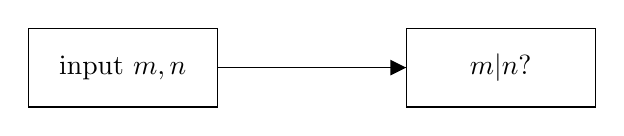
\begin{tikzpicture}[scale=0.2]
			\tikzstyle{every node}+=[inner sep=0pt]
			\draw [black] (0,-2.5) rectangle ++(12,5);
			\draw (6,0) node {input $m,n$};
			\draw [black] (12,0) -- (24,0);
			\fill [black] (24,0) -- (23,0.5) -- (23,-0.5);
			\draw [black] (24,-2.5) rectangle ++(12,5);
			\draw (30,0) node {$m|n$?};
		\end{tikzpicture}
		\caption{ภาพใหญ่ของปัญหาซึ่ง input คือจำนวนนับ $m,n$ และ output คือบอกว่าหารลงตัวหรือไม่}
	\end{center}
\end{figure}
เราจะเริ่มจากนิยามแรกสุดของทฤษฎีจำนวน นั่นคือการหารลงตัวของจำนวนเต็ม ซึ่งจริง ๆ แล้วนั้นเราสามารถตรวจสอบว่าจำนวน 2 จำนวนเช่น $m$ และ $n$ ที่ให้มานั้นหารลงตัวกันหรือไม่ได้โดยง่ายผ่านตัวดำเนินการ ``\%'' ซึ่งเป็นตัวดำเนินการ built-in ของ Python เพื่อหาเศษเหลือจากการหาร โดยตรวจสอบว่าเศษเหลือเป็น 0 หรือไม่ด้วย code ดังนี้
\begin{python*}
m%n == 0
\end{python*}
\noindent โดยที่ code ดังกล่าวจะคืนค่า True ถ้าหารลงตัว และคืนค่า False ถ้าหารไม่ลงตัว

แต่ในที่นี้เราจะเริ่มเขียนฟังก์ชันเพื่อตรวจสอบการหารลงตัวกันด้วยตัวเองก่อนโดยอาศัยนิยามในการออกแบบ โดยสมมติว่าเราจะให้พารามิเตอร์แรกเป็นตัวตั้งและพารามิเตอร์ตัวที่สองเป็นตัวหาร และชื่อฟังก์ชันคือ \texttt{isDivisible} แต่ก่อนจะเริ่มลงมือเขียน code เราจะมาทบทวนนิยามของการหารลงตัวกันอีกรอบ
\boxrule{ทบทวนนิยามการหารลงตัว}{ให้ $m$ และ $n$ เป็นจำนวนเต็ม เราจะกล่าวว่า $m$ หารด้วย $n$ ลงตัว ถ้ามีจำนวนเต็ม $k$ ที่ทำให้ $m=nk$}

จากนิยาม จะเห็นว่าเป้าหมายหลักของฟังก์ชันหลังจากที่รับ $m$ และ $n$ เข้ามาแล้วคือต้องหาว่ามีจำนวนเต็ม $k$ ที่เป็นผลหารดังกล่าวหรือไม่ โดยถ้าดูตามนิยามแล้วจะดูเหมือนว่าเราต้องตรวจสอบหาผลหาร $k$ ไปเรื่อยๆ จนกว่าจะพบ $k$ ที่ทำให้ $m=nk$ ดังนี้
\begin{python*}[Not complete divisibility checking]
k = 1
while m != n*k:
    k += 1
# after exiting from while-loop, k should be an integer such that m = nk,
# i.e. n is a factor of m
\end{python*}
\noindent ทว่า วิธีดังกล่าวจะทำงานไม่รู้จบถ้าค่าที่ได้รับเข้ามาเป็นคู่ที่หารกันไม่ลงตัว เพราะเหตุผลของการหารไม่ลงตัวคือ
\begin{align*}
	m\nmid n
	&\Longleftrightarrow \text{ทุก $k \in \Z$ จะได้ว่า $m \neq nk$}
\end{align*}
กล่าวคือ เราต้องตรวจสอบทุกจำนวนเต็ม $k$ ซึ่งเป็นไปไม่ได้ในการเขียนโปรแกรม อีกทั้ง ถึงแม้ว่าจะหารลงตัวก็ตาม ก็ยังคงมีคำถามว่าแล้วเราจะเริ่มหา $k$ จากไหนและไปทางไหน เพราะถ้าหาผิดทางอาจจะทำงานไม่รู้จบได้เหมือนกัน ตัวอย่างเช่นเราอยากตรวจสอบว่า -10 หารด้วย 5 หรือไม่ ถ้าเราใช้ loop เริ่มจาก $k=1$ และบวก 1 ไปเรื่อย ๆ ดังตัวอย่างข้างบน จะพบว่าโปรแกรมจะทำงานไม่รู้จบเพราะ $k$ ตัวที่ต้องการคือ $k = -2$ ซึ่งไม่อยู่นี้ขอบเขตการหาที่กำหนดไว้

แต่ว่าเรามีคุณสมบัติหนึ่งที่เกี่ยวกับการหารลงตัวที่สามารถจำกัดขอบเขตการหาผลหาร $k$ ได้ ซึ่งกล่าวว่า
\boxrule{คุณสมบัติเพื่อจำกัดขอบเขตของการหารลงตัว}{ให้ $m$ และ $n$ เป็นจำนวนเต็ม ถ้า $m|n$ แล้ว $|n|\leq |m|$}
ซึ่งในทำนองเดียวกัน เราสามารถมองผลหารเป็นตัวประกอบอีกตัวหนึ่งของ $m$ ได้เช่นเดียวกัน จึงได้ว่า $|k| \leq |m|$ กล่าวคือถ้าจะมีผลหารของการหารลงตัวได้นั้น ผลหารดังกล่าวก็จะอยู่ได้แค่ในกลุ่ม $k\in \{-m, -m+1, \dots, -1,0,1, \dots, m-1, m\}$ เพราะฉะนั้น เราจึงจำกัดขอบเขตการหาผลหาร $k$ ได้ไม่ว่าจะหารลงตัวหรือหารไม่ลงตัวก็ตาม กล่าวคือ
\begin{align*}
	m | n
	&\Longleftrightarrow \text{มี $k \in \{-m, -m+1, \dots, m-1, m\}$ ที่ทำให้ $m = nk$}
\end{align*}

\subsection{วิธีเบื้องต้น}
จากนิยามที่ได้กล่าวมานั้น เราสามารถเขียนโปรแกรมเพื่อตรวจสอบการหารลงตัวได้ด้วยการตรวจสอบว่าเจอผลหารหรือไม่ด้วยโปรแกรมดังนี้
\begin{python*}[Check divisibility]
def isDivisible_ver1(m,n):
    qoutList = range(-m,m+1)
    for k in qoutList:
        if m = n*k:
            return True
    return False
\end{python*}
ซึ่งโปรแกรมดังกล่าวจะรันลูปไปเรื่อย ๆ และเมื่อไหร่ก็ตามที่เจอผลหาร ฟังก์ชัน isDivisible จะคืนค่า True มาให้ แต่ถ้ารันจนครบลูปแล้วแต่ไม่เจอผลหาร จะคืนค่า False มาให้ เพราะไม่มีตัวประกอบ
\boxrule{ลองทำดู}{ออกแบบให้จำนวนครั้งการค้นหาลดลงได้หรือไม่ ถ้าทำได้แล้วความซับซ้อนของจำนวนครั้งการค้นหาลดลงหรือไม่}

\subsection{พิจารณาแค่จำนวนบวกก็พอ}
ถ้าลองสังเกตนิยามการหารลงตัวดีๆ จะพบว่าการเป็นจำนวนเต็มบวกหรือจำนวนเต็มลบของตัวตั้งและตัวหารไม่ส่งผลต่อการคิด เพราะเราสามารถเปลี่ยนรูปแบบปัญหาให้พิจารณาแค่กรณีที่ทั้งตัวตั้งและตัวหารเป็นจำนวนเต็มบวกอย่างเดียวได้ เนื่องจากถ้า $m = nk$ แล้วจะได้ว่า
\begin{align*}
	(-m) = nk &\Longleftrightarrow m = n(-k)\\
	m = (-n)k &\Longleftrightarrow m = n(-k)\\
	(-m) = (-n)k &\Longleftrightarrow m = nk
\end{align*}
กล่าวคือ เราทราบการเป็นบวกหรือลบของผลหาร $k$ ได้โดยพิจารณาก่อนว่าตัวตั้งและตัวหารมีเครื่องเหมือนกันหรือแตกต่างกัน และใช้การตรวจสอบการหารลงตัวโดยอาศัยแค่ค่าบวกของ $m$ และ $n$ ที่เป็นตัวตั้งและตัวหาร

แต่เนื่องจากเราต้องการผลลัพธ์ในแง่การหารลงตัวว่าหารลงตัวหรือไม่ ไม่ได้ต้องการค่าผลหาร จึงไม่จำเป็นต้องแบ่งกรณีการคำนวณของโปรแกรมออกตามความเหมือนหรือความต่างของเครื่องหมายของตัวตั้งและตัวหาร กล่าวคือเราสามารถพิจารณาแค่ค่าบวกของทั้งคู่และตัดขอบเขตการหาผลลัพธ์การหารเป็นแค่ $k\in \{1,2, \dots, m-1, m\}$ ซึ่งจะได้โปรแกรมดังนี้
\begin{python*}[Check divisibility by positive]
def isDivisible_ver2(m,n):
    if m < 0:
        m = -m
    if n < 0:
        n = -n
    qoutList = range(1,m+1)
    for k in qoutList:
        if m = n*k:
            return True
    return False
\end{python*}
และโปรแกรมสำหรับการตรวจสอบการหารลงตัวที่จะพัฒนาต่อจากนี้จะขอสมมติว่าเรารับแค่จำนวนเต็มบวกมาตรวจสอบ ซึ่งถ้าจะทำให้รับจำนวนเต็มใด ๆ สามารถทำได้ในทำนองเดียวกันกับ \texttt{isDivisible\_ver2}

\subsection{เปลี่ยนจากปัญหาการคูณเป็นปัญหาการบวก}
จากนิยามการคูณที่กล่าวว่า $k\cdot n := n + n + \cdots + n$ ($k$ พจน์) จะพบว่าเราสามารถเปลี่ยนจากปัญหาการหาผลหาร $k$ เป็นการลองลูปเพื่อเพิ่มพจน์การบวก $n$ ไปเรื่อย ๆ จนกว่าจะมากกว่าหรือเท่ากับ $m$ โดยถ้าสามารถเท่ากับ $m$ ได้จะได้ว่าหารลงตัว แต่ถ้าเกิน $m$ เมื่อไหร่จะได้ว่าหารไม่ลงตัว
\begin{python*}[Check divisibility addition version]
def isDivisible_ver3(m,n):
    product = 0
    while product < m:
        product += n
    if product == m:
        return True
    else:
        return False
\end{python*}
เราสามารถทำได้ในทางกลับกันคือการลบตัวหารออกด้วย $n$ ไปเรื่อยๆ จนกว่าจะได้เศษการหาร (ซึ่งนำไปประยุกต์ใช้ในการหาเศษการหารได้ด้วย)
\begin{python*}[Check divisibility subtraction version]
def isDivisible_ver4(m,n):
    while m >= n:
        m -= n
    if m == 0:
        return True
    else:
        return False
\end{python*}

\subsection{เขียนแบบฟังก์ชันเวียนเกิด} \label{divisibleRecur}
จาก \texttt{isDivisible\_ver4} จะเห็นแนวคิดของการทำปัญหาเดิมซ้ำกัน โดยถ้าเริ่มจากตัวตั้ง $m$ และตัวหาร $n$ เมื่อทำเสร็จไป 1 รอบของลูป จะได้ว่าตัวตั้งจะเปลี่ยนกลายเป็น $m - n$ โดยที่ตัวหารยังคง $n$ เหมือนเดิม ซึ่งจะเห็นว่าแนวคิดดังกล่าวสามารถเขียนเป็นฟังก์ชันเวียนเกิดเป็น \[ \texttt{isDivisible\_recur(m,n)} = \texttt{isDivisible\_recur(m - n,n)} \]
และตามรูปแบบการเขียนอัลกอริทึมเวียนเกิด สิ่งสำคัญคือต้องเขียนขั้นฐานของการคำนวณ ซึ่งคือขั้นที่เราสามารถกำหนดการคำนวณได้ง่าย ๆ โดยจะพบว่า ขั้นฐานของการคำนวณคือขั้นตอนหลังจากหลุดออกจาก while-loop ของ \texttt{isDivisible\_ver4} กล่าวคือ เมื่อตัวตั้ง $m$ ไม่ค่าน้อยกว่าตัวหาร $n$ โดยที่ถ้าตัวตั้งมีค่าเท่ากับ 0 จะหมายความว่าเราสามารถลดค่าตัวตั้งมาเรื่อย ๆ จนหมดได้พอดี หรือก็คือมีเศษเหลือเป็น 0 นั่นคือการหารลงตัว ในทางกลับกัน ถ้าตัวตั้งมีค่ามากกว่า 0 จะหมายถึงการหารไม่ลงตัว ซึ่งสามารถเขียนเป็นเงื่อนไขขั้นฐานได้ดังนี้ \[ \texttt{isDivisible\_recur(m,n)} = \begin{cases}	\texttt{True}&\text{if }m=0\\
\texttt{False}&\text{if }0<m<n
\end{cases}
\] ซึ่งสามารถเขียนเป็นโปรแกรมได้ดังนี้
\begin{python*}[Check divisibility recursion]
def isDivisible_recur(m,n):
    if m < n:
        if m == 0:
            return True
        else:
            return False
    else:
        return isDivisible_recur(m-n,n)
\end{python*}






\newpage
\section{programming: ตรวจสอบการเป็นจำนวนเฉพาะ}
\subsection{วิธีเบื้องต้น}
ในหัวข้อที่แล้ว เราได้เขียนฟังก์ชันเพื่อตรวจสอบการหารลงตัวไป ในหัวข้อนี้เราจะใช้ประโยชน์จากฟังก์ชันดังกล่าวนำมาตรวจสอบการเป็นจำนวนเฉพาะกันบ้าง โดยลักษณะของปัญหายังคงตรงไปตรงมาคือรับจำนวนนับ $n$ เข้ามาแล้วคืนค่าว่าเป็นจำนวนเฉพาะหรือไม่ดังแผนภาพใน Figure \ref{prime_sol1}
\begin{figure}[h]\label{prime_sol1}
\begin{center}
	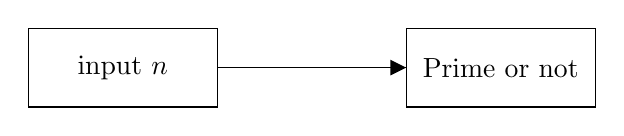
\begin{tikzpicture}[scale=0.2]
		\tikzstyle{every node}+=[inner sep=0pt]
		\draw [black] (0,-2.5) rectangle ++(12,5);
		\draw (6,0) node {input $n$};
		\draw [black] (12,0) -- (24,0);
		\fill [black] (24,0) -- (23,0.5) -- (23,-0.5);
		\draw [black] (24,-2.5) rectangle ++(12,5);
		\draw (30,0) node {Prime or not};
		
	\end{tikzpicture}
	\caption{ภาพใหญ่ของปัญหาซึ่ง input คือจำนวนนับ $n$ และ output คือบอกว่าเป็นจำนวนเฉพาะหรือไม่}
\end{center}
\end{figure}

เริ่มจากทบทวนนิยามของจำนวนเฉพาะ ซึ่งคือ
\boxrule{ทบทวนนิยามจำนวนเฉพาะ}{จำนวนนับ $n$ จะเป็นจำนวนเฉพาะ ถ้ามีเพียงแค่ 1 และ $n$ เท่านั้นที่หาร $n$ ลงตัว}
ซึ่งจากนิยามจะพบว่าเราสามารถตรวจสอบการเป็นจำนวนเฉพาะได้จากการตรวจสอบการหารลงตัวว่าในช่วงตั้งแต่ 1 ถึงจำนวนดังกล่าวมีเพียงแค่ 1 และตัวมันเองเท่านั้นที่หารจำนวนดังกล่าวลงตัว กล่าวคือถ้าเราหาตัวประกอบทั้งหมดของ $n$ ได้ แล้วทำการตรวจสอบว่าเป็นจำนวนเฉพาะหรือไม่ก็จะสามารถตรวจสอบการเป็นจำนวนเฉพาะของ $n$ ได้ทันทีตามแผนภาพใน Figure \ref{prime_sol2}
\begin{figure}[h]\label{prime_sol2}
\centering
		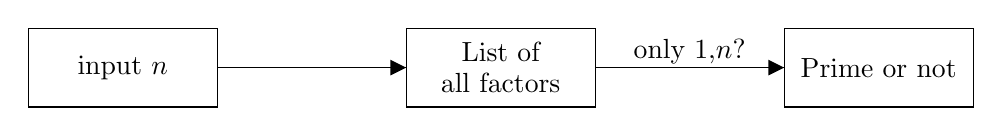
\begin{tikzpicture}[scale=0.2]
			\tikzstyle{every node}+=[inner sep=0pt]
			
			\draw [black] (0,-2.5) rectangle ++(12,5);
			\draw (6,0) node {input $n$};
			\draw [black] (12,0) -- (24,0);
			\fill [black] (24,0) -- (23,0.5) -- (23,-0.5);
			\draw [black] (24,-2.5) rectangle ++(12,5);
			\draw (30,1) node {List of};
			\draw (30,-1) node {all factors};
			
			\draw [black] (36,0) -- (48,0);
			\draw (42,1) node {only 1,$n$?};
			\fill [black] (48,0) -- (47,0.5) -- (47,-0.5);
			\draw [black] (48,0-2.5) rectangle ++(12,5);
			\draw (54,0) node {Prime or not};
		\end{tikzpicture}
		\caption{text}
\end{figure} 
ซึ่่งถ้าเรามีลิสต์ของตัวประกอบของ $n$ แล้วเราจะสามารถเขียนโค้ดเพื่อตรวจสอบการเป็นจำนวนเฉพาะได้ดังนี้
\begin{python*}[Check if it is prime]
# assume we have a list `factorList` which is a list of all factors of n
factorList == [1,n]
\end{python*}

ซึ่งโค้ดดังกล่าวจะให้ค่า True ออกมาถ้า $n$ มีตัวประกอบเพียงแค่ 2 ตัวคือ 1 และ $n$ กล่าวคือ $n$ เป็นจำนวนเฉพาะ แต่ในทางกลับกัน ถ้ามีตัวประกอบอื่นหลงอยู่ในลิสต์ดังกล่าวซึ่งก็คือ $n$ ไม่เป็นจำนวนเฉพาะนั้น จะได้ False ออกมาเป็นผลลัพธ์

\begin{figure}[h]\label{prime_sol3}
	\centering
	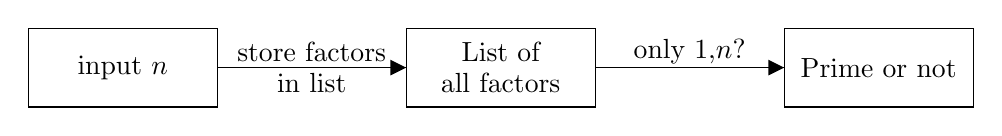
\begin{tikzpicture}[scale=0.2]
		\tikzstyle{every node}+=[inner sep=0pt]
		\draw [black] (0,-2.5) rectangle ++(12,5);
		\draw (6,0) node {input $n$};
		\draw [black] (12,0) -- (24,0);
		\fill [black] (24,0) -- (23,0.5) -- (23,-0.5);
		\draw [black] (24,-2.5) rectangle ++(12,5);
		\draw (30,1) node {List of};
		\draw (30,-1) node {all factors};
		
		\draw [black] (36,0) -- (48,0);
		\draw (42,1) node {only 1,$n$?};
		\fill [black] (48,0) -- (47,0.5) -- (47,-0.5);
		\draw [black] (48,0-2.5) rectangle ++(12,5);
		\draw (54,0) node {Prime or not};
		\draw (18,1) node {store factors};
		\draw (18,-1) node {in list};
	\end{tikzpicture}
	\caption{text}
\end{figure} 

ในตอนนี้เราจะเหลือเพียงแค่ปัญหาของการสร้างลิสต์ของตัวประกอบของ $n$ ซึ่งทำได้โดยง่าย (ใน Python) โดยการรันลูปตั้งแต่ 1 ถึง $n$ และตรวจสอบการเป็นตัวประกอบของ $n$ เพื่อนำไปเก็บใน \texttt{factorList} ทีละตัว ซึ่งทำได้ดังนี้

\begin{python*}[Create factorList]
factorList = []
for m in range(1,n+1):
    if isDivisible(n,m):
        factorList.append(m)
\end{python*}

เมื่อนำโค้ดทั้งสองส่วนมารวมกันและเขียนเป็นฟังก์ชันของ $n$ จะได้
\begin{python}[Check prime]
def isPrime(n):

    factorList = []
    for m in range(1,n+1):
        if isDivisible(n,m):
            factorList.append(m)

    prime = (factorList == [1,n])
    return prime
\end{python}

ทั้งนี้ ยังคงมีคำถามชวนคิดเกี่ยวกับโปรแกรมเช็คจำนวนเฉพาะที่เขียนขึ้นมาว่า
\boxrule{คำถาม}{เพราะเหตุใดเราจึงเขียนลูปแค่บน 1 ถึง $n$ ก็เพียงพอที่จะเช็คการเป็นจำนวนเฉพาะของ $n$ ได้}

จากโปรแกรมที่เขียนมา จะเห็นว่าเราใช้พลังของการมี memory กล่าวคือเราเก็บไว้ก่อนว่ามีใครบ้างเป็นตัวประกอบ แล้วสุดท้ายนำมาตรวจสอบอีกทีว่ามีแค่ 1 และตัวมันเองเท่านั้นที่เป็นตัวประกอบ ซึ่งเราทำการเก็บตัวประกอบไว้ในลิสต์ ซึ่งเป็นเรื่องที่โชคดีที่ลิสต์เป็น built-in data structure ของ Python จึงทำให้เราสามารถ implement วิธีนี้ได้โดยง่าย
ทว่า ในบางภาษานั้นกลับไม่มีลิสต์ให้ใช้ และการตรวจสอบเรื่องการมีใครเป็นสมาชิกบ้างก็ไม่ใช่เรื่องง่ายกับ array ที่เป็นโครงสร้างข้อมูลพื้นฐานในหลาย ๆ ภาษา
ดังนั้น จะแก้ปัญหาอย่างไรถ้าเราอยาก implement โจทย์นี้ในภาษาอื่น ๆ หรือแม้กระทั่งในวิชา Python เองแต่ยังเรียนไม่ถึงการใช้ลิสต์

\subsection{วิธีที่ไม่ใช้ลิสต์ หรือการจำตัวประกอบทั้งหมดของ $n$}
ก่อนอื่น เราจะต้องเปลี่ยนรูปแบบปัญหาให้เป็นปัญหาทางตรรกศาสตร์กันก่อน โดยเริ่มจากนิยามกัน
\begin{align*}
	n>1 \text{ เป็นจำนวนเฉพาะ}
	&\Longleftrightarrow \text{มีเพียงแค่ 1 และ $n$ ที่เป็นตัวประกอบของ $n$}\\
	&\Longleftrightarrow \text{ถ้า $k \notin \{1,n\}$ แล้ว $k$ จะไม่เป็นตัวประกอบของ $n$}\\
	&\Longleftrightarrow \text{ทุก $k=2,...,n-1$ จะได้ว่า $k$ ไม่เป็นตัวประกอบของ $n$}
\end{align*}
หรือในทำนองเดียวกัน เพียงแต่ใช้ความสมมูลเชิงนิเสธ จะได้ว่า
\begin{align*}
	n>1 \text{ ไม่เป็นจำนวนเฉพาะ}
	&\Longleftrightarrow \text{มี $k=2,...,n-1$ ที่ $k$ เป็นตัวประกอบของ $n$}
\end{align*}

กล่าวคือ ถ้าเราจะตรวจสอบว่า $n$ ไม่เป็นจำนวนเฉพาะ เราสามารถทำได้ โดยลูปตั้งแต่ 2 ถึง $n-1$ และเมื่อใดก็ตามที่เจอตัวประกอบเพียงสักตัว เราก็จะสามารถหยุดลูปและบอกได้ทันทีว่า $n$ ไม่เป็นจำนวนเฉพาะ (มาจากการให้เหตุผลว่าประพจน์ $\exists x, P(x)$ เป็นจริง) ซึ่งทำให้เราสามารถเขียนโค้ดได้ดังนี้

\begin{python}[Check prime version2]
def isPrime_ver2(n):

    prime = True               #set as default to be prime
    for k in range(2,n):
        if isDivisible(n,k):   #check if factor
            prime = False      #if k is a factor, set it to be not prime
            break              #stop for loop
    
    return prime
\end{python}

\boxrule{แบบฝึกหัดเพิ่ม}{ลองเขียน \texttt{isPrime\_ver3} โดยใช้ while-loop}
~
\subsection{ลดจำนวนครั้งการคำนวณได้มากกว่านี้อีก}
จากโปรแกรมที่ได้ทำมาแล้วนั้น เราจะพบว่า \texttt{isPrime} มีความซับซ้อนเชิงคำนวณอยู่ที่ $O(n)$ และ \texttt{isPrime\_ver2} มีความซับซ้อนเชิงการคำนวณไม่เกิน $O(n)$ ซึ่งกรณีแย่ที่สุดคือ $n$ ที่เป็นจำนวนเฉพาะ เพราะต้องตรวจสอบทุกจำนวนตั้งแต่ 2 ถึง $n-1$ ว่าเป็นตัวประกอบหรือไม่

ทว่า เราสามารถอาศัยทฤษฎีบทเกี่ยวกับจำนวนเฉพาะที่กล่าวว่า
\boxrule
{การตรวจสอบการเป็นจำนวนเฉพาะโดยตรวจสอบไม่เกิน $\sqrt{n}$ ครั้ง}
{ให้ $n$ เป็นจำนวนนับ ถ้า $p$ ไม่เป็นตัวประกอบของ $n$ สำหรับทุก ๆ จำนวนเฉพาะ $p\leq \sqrt{n}$ แล้ว $n$ จะเป็นจำนวนเฉพาะ}
ถึงแม้ทฤษฎีบทจะบอกว่าเพียงพอที่จะตรวจสอบแค่ตัวประกอบที่เป็นจำนวนเฉพาะที่มีค่าไม่เกิน $\sqrt{n}$ แต่ว่าในการพิจารณากับแค่จำนวน $n$ เพียงจำนวนเดียว เราจะยังคงไม่มีข้อมูลเก่าว่าจำนวนใดบ้างที่เป็นจำนวนเฉพาะ ดังนั้นวิธีที่ง่ายที่สุดคือตรวจสอบกับทุกจำนวนตั้งแต่ 2 ถึง $\lfloor\sqrt{n}\rfloor$ ว่ามีใครบ้างที่เป็นตัวประกอบของ $n$ ซึ่งทำให้เราสามารถแก้โค้ด \texttt{isPrime\_ver2} ให้ตรวจสอบน้อยลงได้ดังนี้

\begin{python}[Check prime version2.1]
import math
def isPrime_ver2_1(n):
    prime = True               #set as default to be prime
    upper = int(math.sqrt(n))
    for k in range(2,upper):
        if isDivisible(n,k):   #check if factor
            prime = False      #if k is a factor, set it to be not prime
            break              #stop for loop
    return prime
\end{python}

\section{programming: แยกตัวประกอบในรูปผลคูณจำนวนเฉพาะ} \label{primeFactor}
หนึ่งในทฤษฎีบทสำคัญของการแยกตัวประกอบของจำนวนเต็มคือ Fundamental Theorem of Arithmetic ซึ่งกล่าวว่า
\boxrule{Fundamental Theorem of Arithmetic}{
	ทุก ๆ จำนวนเต็ม $n$ จะมีจำนวนเฉพาะ $p_1 < p_2 < \dots < p_n$ และจำนวนเต็มบวก $a_1, a_2, \dots, a_n$ เพียงชุดเดียวเท่านั้นที่ทำให้
	$$
	n = p_1^{a_1}p_2^{a_2}\cdots p_n^{a_n}
	$$
	}
ซึ่งเราได้ศึกษาและพิสูจน์ไปแล้วในหัวข้อ \ref{...}

ในหัวข้อนี้ เราจะเขียนโปรแกรมเพื่อหารูปแบบนี้กัน โดยสมมติว่าเราอยากให้โปรแกรมคืนค่าออกมาเป็น dictionary ที่มี keys ระบุจำนวนเฉพาะ และ values ระบุเลขชี้กำลัง ตัวอย่างเช่น $1400=2^3\times 5^2 \times 7$ จะให้ผลลัพธ์ออกมาเป็น \texttt{\{2:3, 5:2, 7:1\}}
\begin{figure}[H]\label{primeFac_sol1}
	\begin{center}
		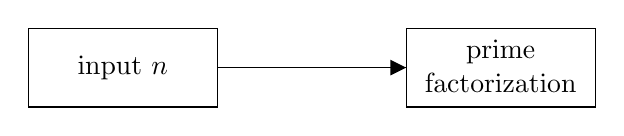
\begin{tikzpicture}[scale=0.2]
			\tikzstyle{every node}+=[inner sep=0pt]
			\draw [black] (0,-2.5) rectangle ++(12,5);
			\draw (6,0) node {input $n$};
			\draw [black] (12,0) -- (24,0);
			\fill [black] (24,0) -- (23,0.5) -- (23,-0.5);
			\draw [black] (24,-2.5) rectangle ++(12,5);
			\draw (30,1) node {prime};
			\draw (30,-1) node {factorization};
		\end{tikzpicture}
		\caption{ภาพใหญ่ของปัญหาซึ่ง input คือจำนวนนับ $n$ และ output คือการแยกตัวประกอบจำนวนเฉพาะที่คืนค่าออกมาเป็น dictionary}
	\end{center}
\end{figure}

\subsection{วิธีวนซ้ำตามจำนวนเฉพาะ}
\subsubsection{ขั้นตอนทำความเข้าใจปัญหา}
จากรูปแบบปัญหา จะเห็นได้โดยง่ายว่าวิธีที่พื้นฐานที่สุดที่ทำได้คือการวนซ้ำไปตามตัวประกอบจำนวนเฉพาะเพื่อหาว่าจะสามารถแยกตัวประกอบจำนวนเฉพาะนั้นออกมาได้กี่รอบ กล่าวคือเราสามารถแยกย่อยปัญหาดังกล่าวออกมาเป็นปัญหาย่อยของทีละจำนวนเฉพาะที่เป็นตัวประกอบ โดยเป็นโจทย์ย่อยว่า

\begin{center}
	กำหนดจำนวนนับ $n$ และจำนวนเฉพาะ $p$\\
	เขียนโปรแกรมเพื่อหาว่าสามารถแยกตัวประกอบ $p$ นั้นออกมาได้กี่ตัว\\
	พูดอีกนัยหนึ่งคือ จงหาจำนวนนับ $k$ ที่ทำให้ $n = p^k\cdot A$ โดยที่ $p\nmid A$
\end{center}

\noindent และเขียนแผนภาพการแก้ปัญหาได้แบบแแผนภาพ \ref{primeFac_sol2}
\begin{figure}[H]
	\begin{center}
		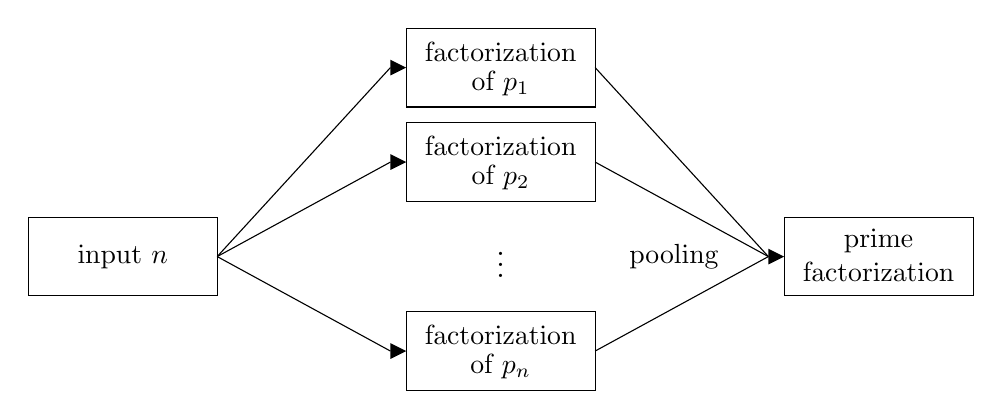
\begin{tikzpicture}[scale=0.2]
			\tikzstyle{every node}+=[inner sep=0pt]
			\draw [black] (0,-2.5) rectangle ++(12,5);
			\draw (6,0) node {input $n$};
			
			\draw [black] (24,-8.5) rectangle ++(12,5);
			\draw [black] (12,0) -- (23,-6);
			\fill [black] (24,-6) -- (23,-5.5) -- (23,-6.5);
			\draw (30,-5) node {factorization};
			\draw (30,-7) node {of $p_n$};
			
			\draw (30,0) node {{\large $\vdots$}};
			\draw [black] (24,3.5) rectangle ++(12,5);
			\draw [black] (12,0) -- (23,6);
			\fill [black] (24,6) -- (23,5.5) -- (23,6.5);
			\draw (30,7) node {factorization};
			\draw (30,5) node {of $p_2$};
			
			\draw [black] (24,9.5) rectangle ++(12,5);
			\draw [black] (12,0) -- (23,12);
			\fill [black] (24,12) -- (23,12.5) -- (23,11.5);
			\draw (30,13) node {factorization};
			\draw (30,11) node {of $p_1$};
			
			\draw [black] (47,0) -- (36,12);
			\draw [black] (47,0) -- (36,6);
			\draw [black] (47,0) -- (36,-6);
			\draw (41,0) node {pooling};
			\fill [black] (48,0) -- (47,0.5) -- (47,-0.5);
			\draw [black] (48,-2.5) rectangle ++(12,5);
			\draw (54,1) node {prime};
			\draw (54,-1) node {factorization};
		\end{tikzpicture}
		\caption{...}\label{primeFac_sol2}
	\end{center}
\end{figure}

ทว่า จะพบว่ายังเหลือปัญหาย่อยที่ว่ามีจำนวนเฉพาะใดบ้างที่เป็นตัวประกอบของ $n$ เพื่อที่จะระบุขอบเขตการแก้ปัญหาย่อย $p_1,\dots,p_n$ ดังนั้นก่อนที่จะแก้ปัญหาย่อยการแยกตัวประกอบจำนวนเฉพาะที่กำหนดตัวประกอบจำนวนเฉพาะมาแล้วนั้น เราจะต้องแก้ปัญหาการหาตัวประกอบที่เป็นจำนวนเฉพาะทั้งหมดของ $n$ ก่อน จึงได้แผนภาพการแก้ปัญหาดังแผนภาพ \ref{primeFac_sol3}

\begin{figure}[H]
	\begin{center}
		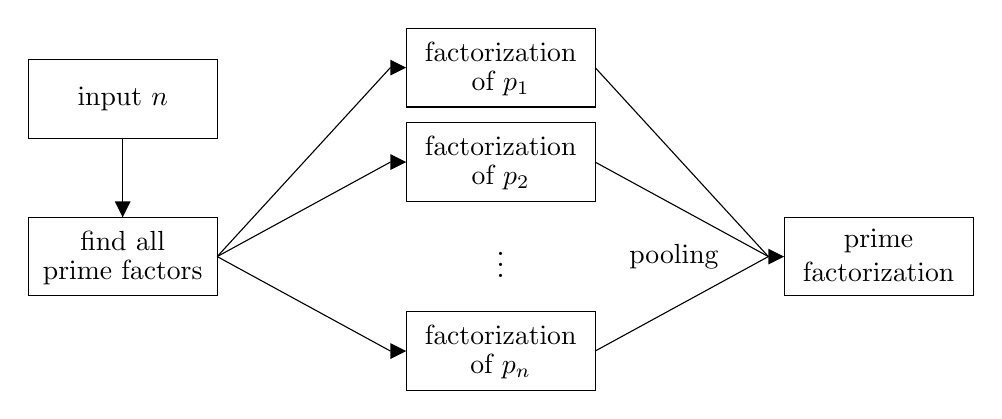
\begin{tikzpicture}[scale=0.2]
			\tikzstyle{every node}+=[inner sep=0pt]
			\draw (6,10) node {input $n$};
			\draw [black] (0,-2.5) rectangle ++(12,5);
			\draw (6,1) node {find all};
			\draw (6,-1) node {prime factors};
			\draw [black] (0,7.5) rectangle ++(12,5);
			\draw [black] (6,7.5) -- (6,2.5);
			\fill [black] (6,2.5) -- (5.5,3.5) -- (6.5,3.5);
			\draw [black] (24,-8.5) rectangle ++(12,5);
			\draw [black] (12,0) -- (23,-6);
			\fill [black] (24,-6) -- (23,-5.5) -- (23,-6.5);
			\draw (30,-5) node {factorization};
			\draw (30,-7) node {of $p_n$};
			
			\draw (30,0) node {{\large $\vdots$}};
			\draw [black] (24,3.5) rectangle ++(12,5);
			\draw [black] (12,0) -- (23,6);
			\fill [black] (24,6) -- (23,5.5) -- (23,6.5);
			\draw (30,7) node {factorization};
			\draw (30,5) node {of $p_2$};
			
			\draw [black] (24,9.5) rectangle ++(12,5);
			\draw [black] (12,0) -- (23,12);
			\fill [black] (24,12) -- (23,12.5) -- (23,11.5);
			\draw (30,13) node {factorization};
			\draw (30,11) node {of $p_1$};
			
			\draw [black] (47,0) -- (36,12);
			\draw [black] (47,0) -- (36,6);
			\draw [black] (47,0) -- (36,-6);
			\draw (41,0) node {pooling};
			\fill [black] (48,0) -- (47,0.5) -- (47,-0.5);
			\draw [black] (48,-2.5) rectangle ++(12,5);
			\draw (54,1) node {prime};
			\draw (54,-1) node {factorization};
		\end{tikzpicture}
		\caption{...}\label{primeFac_sol3}
	\end{center}
\end{figure}

ซึ่งปัญหาย่อยของการแยกตัวประกอบของแต่ละตัวประกอบเฉพาะนั้น เราสามารถใช้ for-loop เพื่อลูปการแก้ปัญหาตามตัวประกอบเฉพาะทั้งหมดที่หามาได้และเก็บผลลัพธ์มาสะสมไว้ ซึ่งจะได้ดังแผนภาพ \ref{primeFac_sol4}
\begin{figure}[H]
	\begin{center}
		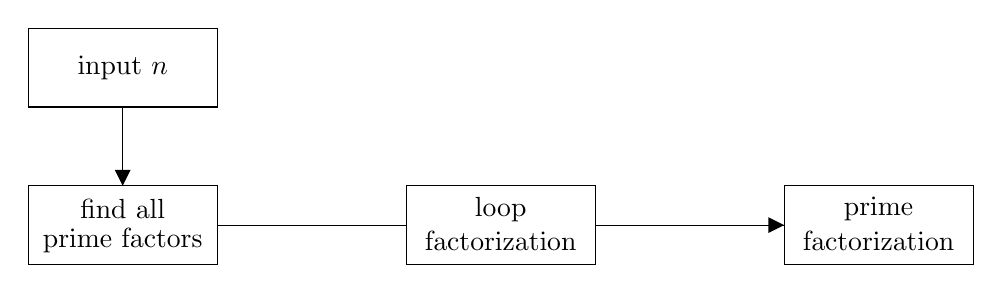
\begin{tikzpicture}[scale=0.2]
			\tikzstyle{every node}+=[inner sep=0pt]
			\draw (6,10) node {input $n$};
			\draw [black] (0,-2.5) rectangle ++(12,5);
			\draw (6,1) node {find all};
			\draw (6,-1) node {prime factors};
			\draw [black] (0,7.5) rectangle ++(12,5);
			\draw [black] (6,7.5) -- (6,2.5);
			\fill [black] (6,2.5) -- (5.5,3.5) -- (6.5,3.5);
			\draw [black] (12,0) -- (24,0);
			\draw [black] (24,-2.5) rectangle ++(12,5);
			\draw (30,1) node {loop};
			\draw (30,-1) node {factorization};
			\draw [black] (36,0) -- (48,0);
			\fill [black] (48,0) -- (47,0.5) -- (47,-0.5);
			\draw [black] (48,-2.5) rectangle ++(12,5);
			\draw (54,1) node {prime};
			\draw (54,-1) node {factorization};
		\end{tikzpicture}
		\caption{...}\label{primeFac_sol4}
	\end{center}
\end{figure}

ทั้งนี้ โจทย์ปัญหาของการหาตัวประกอบที่เป็นจำนวนเฉพาะทั้งหมดของ $n$ จะทิ้งไว้ให้ผู้อ่านทำเป็นแบบฝึกหัดในแบบฝึกหัด \ref{allPrimeFactor} แต่เราจะมาแก้ปัญหาเรื่องจำนวนครั้งการเป็นตัวประกอบของตัวประกอบเฉพาะที่กำหนดมาให้กัน

\subsubsection{แก้ปัญหาย่อยจำนวนครั้งการหารลงตัว}
ก่อนลงรายละเอียด จะขอทบทวนปัญหาอีกสักครั้ง
\begin{center}
	กำหนดจำนวนนับ $n$ และจำนวนเฉพาะ $p$\\
	เขียนโปรแกรมเพื่อหาว่าสามารถแยกตัวประกอบ $p$ นั้นออกมาได้กี่ตัว\\
	พูดอีกนัยหนึ่งคือ จงหาจำนวนนับ $k$ ที่ทำให้ $n = p^k\cdot A$ โดยที่ $p\nmid A$
\end{center}
\begin{figure}[H]\label{subPrimeFac_sol1}
	\begin{center}
		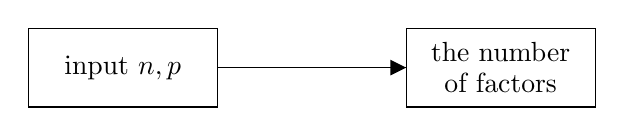
\begin{tikzpicture}[scale=0.2]
			\tikzstyle{every node}+=[inner sep=0pt]
			\draw [black] (0,-2.5) rectangle ++(12,5);
			\draw (6,0) node {input $n, p$};
			\draw [black] (12,0) -- (24,0);
			\fill [black] (24,0) -- (23,0.5) -- (23,-0.5);
			\draw [black] (24,-2.5) rectangle ++(12,5);
			\draw (30,1) node {the number};
			\draw (30,-1) node {of factors};
		\end{tikzpicture}
		\caption{ภาพใหญ่ของปัญหาย่อยซึ่ง input คือจำนวนนับ $n$ และจำนวนเฉพาะ $p$ และ output คือจำนวนครั้งการหาร $n$ ลงตัวของ $p$}
	\end{center}
\end{figure}
ปัญหานี้เป็นปํญหาที่ค่อนข้างง่าย เราสามารถทำได้ด้วยการวนลูปหารซ้ำไปเรื่อย ๆ ด้วยเงื่อนไขว่า ``ตราบใดที่ยังหารลงตัวอยู่ (\texttt{n\%p == 0}) ให้หารต่อ'' และทุกครั้งการหารเราจะมีตัวแปรเพื่อเก็บจำนวนครั้งการหารไว้ (\texttt{counter += 1}) และอัพเดตตัวตั้งการหารเป็นผลหารล่าสุด \texttt{n = n//p} ซึ่งสามารถเขียนเป็นโค้ดได้ดังนี้
\begin{python*}[factorization of given prime $p$]
def countFactor(n,p):
    count = 0
    while n%p == 0:
        count += 1
        n = n//p
    return count
\end{python*}

\subsubsection{รวบรวมวิธีแก้ปัญหาย่อยเพื่อแก้ปัญหาหลัก}
ตอนนี้เรามีฟังก์ชัน \texttt{countFactor} เพื่อช่วยในการนับจำนวนตัวประกอบเฉพาะ $p$ ของ $n$ และ(สมมติ)มีฟังก์ชัน \texttt{findAllPrimeFactor} เพื่อช่วยในการหาตัวประกอบเฉพาะทั้งหมดของ $n$ หรือพูดอีกนัยหนึ่งคือ เราสามารถหาได้แล้วว่าเมื่อทำการแยกตัวประกอบเฉพาะของ $n$ จะมีจำนวนเฉพาะใดคูณกันอยู่บ้าง และแต่ละจำนวนเฉพาะดังกล่าวมีเลขชี้กำลังเป็นอะไร ตอนนี้เหลือเพียงแค่นำ 2 ฟังก์ชันดังกล่าวมาทำงานร่วมกันตามแผนที่วางไว้ในแผนภาพ \ref{primeFac_sol4} ซึ่งเราจะสามารถเขียนโค้ดได้ดังนี้
\begin{python}[Prime Factorization]
def primeFactorize(n):
    primeList = findAllPrimeFactor(n)
    resultDict = {}
    for p in primeList:
        resultDict[p] = countFactor(n,p)
    return resultDict
\end{python}

\subsection{วิธีเวียนเกิด}
ถ้าลองสังเกตวิธีคำนวณของฟังก์ชัน \texttt{countFactor} ดี ๆ จะพบว่ามีแนวคิดของการเรียกฟังก์ชันแบบเวียนเกิดที่สำคัญอยู่อย่างหนึ่ง ซึ่งคือการที่เราไม่ได้พิจารณาตัวตั้งของการหารว่ามีค่า $n$ ที่รับมาตลอดเวลา แต่ $n$ ในการพิจารณารอบถัดไปก็เกิดจากการที่เราตัดทอนตัวประกอบที่หาพบมาแล้วหนึ่งตัว ($n/p$) ซึ่งถึงแม้ว่าในฟังก์ชันดังกล่าวจะทำอยู่กับแค่ $p$ ตัวเดียว แต่เราก็สามารถขยายแนวคิดนี้มาสู่กรณีใด ๆ ที่ไม่ได้กำหนดตัวประกอบเฉพาะตายตัวไว้ได้เช่นกัน

จากประเด็นดังกล่าว จึงนำมาสู่แนวคิดการออกแบบในรูปแบบเวียนเกิดว่า เราให้ฟังก์ชันนั้นหยิบตัวประกอบเฉพาะที่เล็กที่สุดออกมาก่อนหนึ่งตัว ($p_1$) แล้วปล่อยให้ฟังก์ชันเดิมคำนวณกับกรณี $n/p_1$ จนกว่าจะได้ว่าหารแล้วเหลือแค่ 1 ซึ่งมาจากแนวคิด
\[ n = \underbrace{p_1^{a_1}p_2^{a_2}\cdots p_n^{a_n}}_\texttt{algor(n)} = p_1 \times (\underbrace{p_1^{a_1 - 1}p_2^{a_2}\cdots p_n^{a_n}}_\texttt{algor(n/p\_1)}) = p_1 \times (n/p_1)\]

ทว่า สิ่งที่เราต้องการทำคือการเก็บจำนวนครั้งการหารลงตัวไว้ใน dictionary ดังนั้นเราจึงต้องให้อัลกอริทึมที่เรากำลังจะสร้างคืนค่าเป็น dictionary ของจำนวนครั้งการหารลงตัวของ $n/p_1$ และทำการอัพเดต $p_1$ เพิ่มเข้าไปอีก 1 ครั้ง ซึ่งสามารถทำได้ง่ายผ่านคำสั่ง \texttt{dict[key] = dict.get(key,0) + 1} (ถ้าไม่มี key นั้นให้คืนค่า 0 แล้วเพิ่มไป 1 จึงได้ 1 แต่ถ้ามี key นั้นอยู่แล้วให้คืนค่าเดิมออกมาก่อนแล้วบวกเพิ่มไปอีก 1 แล้วบันทึกกับลงไปใน key เดิม)

นอกจากนั้น ยังพบว่าเครื่องมืออีกชิ้นที่สำคัญของแนวคิดนี้คือการหาตัวประกอบเฉพาะที่มีค่าน้อยที่สุดก่อน ซึ่งสามารถปรับปรุงจากฟังก์ชันที่เขียนเป็นแบบฝึกหัดข้อ \ref{allPrimeFactor} โดยให้คำนวณจากน้อยไปมาก และเมื่อเจอตัวประกอบเฉพาะตัวแรกก็ให้คืนค่าทันที โดยในที่นี้ขอสมมติชื่อฟังก์ชันเป็น \texttt{minPrimeFactor}

สุดท้าย จะสามารถเขียนโค้ดได้ดังนี้
\begin{python}[Recursive Prime Factorization]
def primeFactorize_recur(n):
    if n == 1:
        return {}
    else:
        min_p = minPrimeFactor(n)
        result_dic_recur = primeFactorize_recur(n//min_p)
        result_dic_recur[min_p] = result_dic_recur.get(min_p,0) + 1
        return result_dic_recur
\end{python}

\section{programming: ขั้นตอนวิธีการหารหาเศษและผลหาร} \label{prog:divisionAlgo}

\newpage
\section{Programming Exercise}
\begin{enumerate}
	\item จงวิเคราะห์ความซับซ้อนของอัลกอริทึมต่าง ๆ ในการตรวจสอบการหารลงตัว ทั้งรูปแบบเชิงทฤษฎี และเชิงการทดลองเพื่อเปรียบเทียบ โดยที่สมมติว่าทุก operation (บวก ลบ คูณ การเปรียบเทียบ) มีต้นทุนเท่ากับ 1 หน่วย
	\item โปรแกรม \texttt{isDivisible\_recur} ที่ให้เป็นตัวอย่างในหัวข้อ \ref{divisibleRecur} ยังคงอยู่ภายใต้เงื่อนไขว่าใส่ได้แค่จำนวนเต็มบวก จงพิจารณาว่าเราสามารถแก้ไขให้รับกับจำนวนเต็มใด ๆ ด้วยวิธีเดียวกับ \texttt{isDivisible\_ver2} ได้หรือไม่เพราะเหตุใด ถ้าไม่ได้จงหาวิธีแก้ไขวิธีอื่น
	\item จงเขียนโปรแกรมเพื่อหาผลหารและเศษเหลือจากขั้นตอนวิธีการหาร
	\item จงเขียนโปรแกรมตรวจสอบการเป็นจำนวนเฉพาะโดยใช้รูปแบบเวียนเกิด
	\item จงเขียนโปรแกรมที่รับจำนวนนับ $n$ และคืนค่าลิสต์ของทุกจำนวนเฉพาะตั้งแต่ 1 ถึง $n$ โดยที่แย่ที่สุดไม่เกิน $O(nูู^\frac{3}{2})$\\
	(เราสามารถทำได้ง่ายที่สุดคือ $O(n^2)$ ด้วยการตรวจสอบทีละจำนวนว่าเป็นจำนวนเฉพาะหรือไม่ด้วยวิธี ver2 และ print เมื่อเป็นจำนวนเฉพาะ)
	\item \label{allPrimeFactor} จงเขียนโปรแกรมที่รับจำนวนนับ $n$ และคืนค่าเป็นลิสต์ของจำนวนเฉพาะที่เป็นตัวประกอบของ $n$ 
	\item จงเขียนฟังก์ชันนับจำนวนครั้งการหาร $n$ ด้วย $p$ ลงตัว (ฟังก์ชัน \texttt{countFactor}) แบบเวียนเกิด 
	\item จงเขียนโปรแกรมที่รับจำนวนนับ $n$ และคืนค่าจำนวนของตัวประกอบที่เป็นบวกทั้งหมดของ $n$
	\item \label{primeFactFac} จงเขียนฟังก์ชันที่รับจำนวนนับ $n$ และคืนค่าออกมาเป็น dictionary ของการแยกตัวประกอบเฉพาะของ $n!$ (caution: จะพบว่าเราสามารถแก้ปัญหาโดยอาศัยฟังก์ชัน \texttt{primeFactorize} ในหัวข้อ \ref{primeFactor} ได้โดยง่าย แต่ว่าจะมีปัญหาเมื่อ $n$ มีค่าใหญ่ ๆ จนทำให้การเก็บ $n!$ ใช้หน่วยความจำเกิน)
	\item อาศัยฟังก์ชันที่เขียนขึ้นมาในแบบฝึกหัดข้อ \ref{primeFactFac} เพื่อเขียนฟังก์ชันที่รับจำนวนนับ $n$ แล้วคืนค่าเป็นจำนวนของเลข 0 ที่ลงท้ายของผลลัพธ์ของ $n!$
\end{enumerate}

   	\chapter{Combinations}

\begin{center}
	   \title{\sffamily\colorbox{black}{\bfseries\textcolor{white}{\Large THEORY PART}}}
\end{center}

ในบทนี้จะกล่าวถึงเทคนิคต่าง ๆ เกี่ยวกับการนับจำนวนเหตุการณ์ โดยเริ่มจากเทคนิคเบื้องต้นที่สุดซึ่งคือหลักการบวกและหลักการคูณที่เป็นพื้นฐานของสูตรการนับอื่น ๆ ที่จะกล่าวถึงต่อไปในบทนี้ กล่าวคือถึงแม้เราจะไม่รู้สูตรในการคำนวณการนับแบบยาก ๆ แต่ถ้าเราใช้ทักษะด้านการวางแผนช่วยในการนับ ทุกปัญหาจะสามารถถูกแก้ปัญหาได้โดยใช้เพียงแค่หลักการบวกและหลักการคูณได้ หลังจากทำความคุ้นเคยกับการวางแผนการนับเหตุการณ์เบื้องต้นด้วยหลักการบวกและหลักการคูณแล้ว จะเริ่มกล่าวถึงสูตรของรูปแบบการนับต่าง ๆ ที่เฉพาะเจาะจงมากขึ้น ได้แก่ การเรียงสับเปลี่ยน และการจัดกลุ่ม ทั้งในรูปแบบไม่มีของซ้ำกันและมีของซ้ำกันหรือเลือกซ้ำได้

\section{หลักการบวกและหลักการคูณ}

~\indent อย่างที่ได้กล่าวไปตอนต้นว่าทุกสูตรที่จะถูกกล่าวถึงในบทนี้นั้นมีแนวคิดตั้งต้นมาจากหลักการบวกและหลักการคูณทั้งสิ้น เพียงแต่ต้องอาศัยทักษะในการวางแผนการนับให้เป็นขั้นเป็นตอน ดังนั้นจุดประสงค์ของหัวข้อนี้คือการทำความคุ้นเคยกับการวางแผนการนับผ่านโจทย์ที่อยู่ในระดับง่ายถึงปานกลาง โดยที่เครื่องมือการนับในเวลานี้มีเพียงแค่หลักการบวกและหลักการคูณ

\subsection{หลักการบวก}
\boxrule{หลักการบวก\index{หลักการบวก}\index{additive rule}}{ในการทำงานอย่างหนึ่งมีทางเลือกการทำอยู่ 2 ทางเลือก โดยที่ทางเลือกแรกมีวิธีทำได้ $ p $ วิธีแตกต่างกัน และทางเลือกที่สองมีวิธีทำได้ $ q $ วิธีแตกต่างกัน โดยที่ทางเลือกทั้งสองไม่มีวิธีการทำร่วมกัน และเลือกทำได้แค่ทางเลือกใดทางเลือกหนึ่งเท่านั้น ถ้าต้องการเลือกวิธีการทำงานชิ้นนี้จะสามารถเลือกทำได้ $ p+q $ วิธีที่แตกต่างกัน}

สิ่งแรกที่ต้องนึกถึงเมื่อจะเลือกใช้หลักการบวกคือกระบวนการนับของเราเป็นการแยกกรณี กล่าวคือเป็นทางเลือกให้ทำเพียงอย่างใดอย่างหนึ่ง โดยที่ไม่ว่าจะเลือกทำทางไหนก็ถือว่าจบกระบวนการทำงานชิ้นนั้น และอย่างที่สองที่ต้องระวังคือทางเลือกที่แยกออกไปต้องไม่มีวิธีการที่ซ้ำกัน กล่าวคือไม่มีการนับซ้ำเกิดขึ้นในกระบวนการนับ

ในส่วนของโจทย์ด้านล่างนั้น ผู้อ่านคงทราบดีว่าเราต้องใช้หลักการบวกในการนับเพราะเป็นโจทย์ในหัวข้อหลักการบวก แต่สิ่งที่ผมอยากให้ผู้อ่านนึกหลังจากอ่านโจทย์เสร็จคืออะไรเป็นคีย์เวิร์ดสำคัญที่บอกเราว่าขั้นตอนนี้ต้องใช้หลักการบวก

\begin{exam}
	มหาวิทยาลัยแห่งหนึ่งมีนิสิตวิชาเอกคณิตศาสตร์ 33 คน และมีนิสิตวิชาเอกวิทยาการคอมพิวเตอร์ 40 คน ถ้าต้องการเลือกนักศึกษาหนึ่งคนเพื่อเป็นคณะกรรมการของสโมสรนิสิต จะมีวิธีเลือกนิสิตดังกล่าวได้แตกต่างกันกี่วิธี
\end{exam}
\solution{...}


\begin{exam} \label{addSet}
	ให้เซต $ A=\{a,b,c,d\} $ และ $ B=\{\alpha,\beta,\gamma\} $ ถ้าต้องการเลือกตัวอักษรหนึ่งตัวจากเซต $ A $ หรือเซต $ B $ จะมีวิธีเลือกได้กี่วิธี
\end{exam}
\solution{...}

นอกจากที่เรากล่าวถึงหลักการบวกในแง่เปรียบเทียบกับการเลือกวิธีการทำงานในรูปแบบภาษามนุษย์แล้วนั้น จากตัวอย่างที่ \ref{addSet} เราจะพบว่าเราสามารถนิยามหลักการบวกได้โดยใช้เซตเข้ามาช่วยในการพูดให้เป็นภาษาคณิตศาสตร์มากขึ้นได้ดังนี้\\

\boxrule{หลักการบวกแบบภาษาเซต}{กำหนดให้ $ A $ และ $ B $ เป็นเซตที่มีสมาชิกแตกต่างกัน กล่าวคือ $ A\cap B = \emptyset $ จะได้ว่า $$ \left|A\cup B\right| = \left| A \right|+\left| B \right| $$}

และนอกจากที่เรานิยามหลักการบวกโดยใช้แค่ 2 ทางเลือก เรายังสามารถขยายแนวคิดออกไปให้มีมากกว่า 2 ทางเลือกได้ในทำนองเดียวกันคือ\\

\boxrule{หลักการบวกกรณีทั่วไป}{ถ้ามีทางเลือก $ m $ ทางเลือก ซึ่งไม่มีทางเลือกใดที่มีวิธีการซ้ำกับทางเลือกอื่น ๆ สมมติว่าทางเลือกที่หนึ่งมีวิธีทำได้ $ r_1 $ วิธี ทางเลือกที่สองมีวิธีทำได้ $ r_2 $ วิธี $ \dots $ และทางเลือกที่ $ m $ มีวิธีทำได้ $ r_m $ วิธี ดังนั้นจะมีวิธีเลือกทำงานชิ้นนี้เพียงอย่างใดอย่างหนึ่งได้แตกต่างกัน $ r_1+r_2+\cdots+r_m $ วิธี\\
	
	หรือกล่าวแบบภาษาเซตคือ ถ้า $ A_1, \dots, A_m $ เป็นเซตที่ไม่มีสองเซตใด ๆ ที่มีสมาชิกร่วมกัน กล่าวคือ $ A_i\cap A_j = \emptyset $ สำหรับทุก ๆ $ i\neq j $ จะได้ว่า $$ \left| A_1 \cup \cdots \cup A_m \right| = \left| A_1 \right| + \cdots + \left| A_m \right| $$}

\begin{exam}
	จงหา $ \left| \left\{ (x,y) \in \Z\times\Z \colon x^2+y^2\leq 4 \right\} \right| $
\end{exam}
\solution{...}
\subsection{หลักการคูณ}

\boxrule{หลักการคูณ\index{หลักการคูณ}\index{multiplicative rule}}{กระบวนการทำงานอย่างหนึ่งประกอบด้วยขั้นตอนย่อยๆ สองขั้นตอน โดยขั้นตอนแรกมีวิธีทำได้แตกต่างกัน $ p $ วิธี และไม่ว่าจะเลือกวิธีใดก็ตามในขั้นตอนแรกจะสามารถทำขั้นตอนที่สองได้แตกต่างกัน $ q $ วิธี และขั้นตอนทั้งสองนี้ไม่สามารถทำงานร่วมกันได้ ดังนั้นจะมีวิธีทำงานชิ้นนี้ได้แตกต่างกัน $ pq $ วิธี}

ประเด็นสำคัญของหลักการคูณคือการที่งานชิ้นนั้นมีความเป็นขั้นตอนทำอย่างต่อเนื่องกัน และต้องทำทุกขั้นตอนถึงจะเสร็จงานชิ้นนั้น ถ้าในการวางแผนการนับมีการแบ่งการนับออกเป็นขั้นและมั่นใจว่าเมื่อทำจบทุกขั้นแล้วจะได้ผลลัพธ์ของการจัดเรียงออกมาตามที่เราต้องการก็เป็นการยืนยันได้ในระดับหนึ่งว่าเราจะต้องใช้หลักการคูณเข้ามานับ นอกจากนั้น ข้อระวังของกฏการคูณที่ต้องพึงระวังไว้เสมอคือจำนวนวิธีการเลือกทำในขั้นตอนถัดไปจะต้องเท่ากันทั้งหมดไม่ว่าจะเลือกทำวิธีการใดในขั้นตอนปัจจุบันก็ตาม กล่าวเทียบกับนิยามด้านบนคือ ไม่ว่าเราจะเลือกวิธีใดใน $ p $ วิธีของขั้นตอนที่หนึ่ง เราจะต้องสามารถทำขั้นตอนที่สองได้ $ q $ วิธีทั้งหมด\\

\boxnote{คำถาม}{จริง ๆ แล้วเราสามารถมองหลักการคูณจากมุมมองของหลักการบวกได้ ซึ่งจะพบเหตุผลว่าทำไมเงื่อนไขของการที่จำนวนวิธีที่เลือกทำได้ในขั้นตอนถัดไปต้องเท่ากันไม่ว่าเลือกทำวิธีใดมาเป็นเงื่อนไขที่สำคัญ จงพิจารณาหลักการคูณโดยใช้การอธิบายในรูปแบบของหลักการบวก}

\begin{exam}
	มหาวิทยาลัยแห่งหนึ่งมีนิสิตวิชาเอกคณิตศาสตร์ 33 คน และมีนิสิตวิชาเอกวิทยาการคอมพิวเตอร์ 40 คน ถ้าต้องการเลือกนักศึกษาสองคนจากวิชาเอกละหนึ่งคนเพื่อเป็นคณะกรรมการของสโมสรนักศึกษา จะมีวิธีเลือกนักศึกษาได้แตกต่างกันกี่วิธี
\end{exam}
\solution{...}
\begin{exam}
	ให้เซต $ A=\{a,b,c,d\} $ และ $ B=\{\alpha,\beta,\gamma\} $ ถ้าต้องการเลือกตัวอักษร 2 ตัวจากเซต $ A $ และเซต $ B $ เซตละหนึ่งตัว จะมีวิธีเลือกที่แตกต่างกันกี่วิธี
\end{exam}
\solution{...}
ในทำนองเดียวกัน หลักการคูณก็สามารถเขียนได้ในรูปแบบของเซตดังนี้\\

\boxrule{หลักการคูณแบบภาษาเซต}{กำหนดให้ $ A $ และ $ B $ เป็นเซต และ $ A\times B = \left\{ (a,b) \colon a\in A, b\in B \right\} $ แล้วจะได้ว่า $$ \left|A\times B\right| = \left| A \right|\times\left| B \right| $$}

\begin{exam}
	จำนวนเต็มคี่ที่อยู่ระหว่าง 1000 และ 10000 ซึ่งมีเลขในแต่ละหลักแตกต่างกันมีทั้งหมดกี่จำนวน
\end{exam}
\solution{...}
\boxrule{หลักการคูณกรณีทั่วไป}{ถ้างานชิ้นหนึ่งประกอบด้วย $ m $ ขั้นตอน สมมติว่าขั้นตอนที่หนึ่งมีวิธีทำได้ $ r_1 $ วิธี ขั้นตอนที่สองมีวิธีทำได้ $ r_2 $ วิธีไม่ว่าจะเลือกวิธีการใดในขั้นตอนที่หนึ่งก็ตาม $ \dots $ และขั้นตอนที่ $ m $ มีวิธีทำได้ $ r_m $ วิธีไม่ว่าจะเลือกวิธีการใดในขั้นตอนก่อนหน้าก็ตาม ดังนั้นจะมีวิธีเลือกทำงานชิ้นนี้ได้แตกต่างกัน $ r_1 \times r_2\times\cdots\times r_m $ วิธี\\
	
	หรือกล่าวแบบภาษาเซตคือ ถ้า $ A_1, \dots, A_m $ เป็นเซตใด ๆ แล้วจะได้ว่า $$ \left| A_1 \times \cdots \times A_m \right| = \left| A_1 \right| \times \cdots \times \left| A_m \right| $$}

%\subsection{แบบฝึกหัดเพิ่มเติม}
\begin{exam}
	จำนวนเต็มคู่ที่อยู่ระหว่าง 1000 และ 10000 ซึ่งมีเลขในแต่ละหลักแตกต่างกันมีทั้งหมดกี่จำนวน
\end{exam}
\solution{...}

\begin{exam}
	จงแสดงว่าเซตที่มีสมาชิก $ n $ ตัวมีเซตย่อย $ 2^n $ เซต
\end{exam}
\solution{...}

\begin{exam}
	มีคู่สามีภรรยา 15 คู่ในงานปาร์ตีแห่งหนึ่ง จงหาจำนวนวิธีการเลือกผู้หญิงหนึ่งคนและผู้ชายอีกหนึ่งคนโดยที่ (1) ต้องเป็นคู่สามีภรรยากัน (2) ต้องไม่เป็นคู่สามีภรรยากัน
\end{exam}
\solution{...}

\begin{exam}
	พาสเวิร์ดของระบบความปลอดภัยแห่งหนึ่งเป็นตัวอักษรภาษาอังกฤษยาว 3 หรือ 4 ตำแหน่ง จงหา (1) จำนวนของพาสเวิร์ดที่เป็นไปได้ทั้งหมด (2) จำนวนของพาสเวิร์ดที่เป็นไปได้ทั้งหมดที่ใช้ตัวอักษรไม่ซ้ำกัน
\end{exam}
\solution{...}

\begin{exam}
	จงหาจำนวนของตัวประกอบที่เป็นจำนวนเต็มบวกของ $441,000 ( =2^3\times 3^2 \times 5^3 \times 7^2 )$
\end{exam}
\solution{...}

%\boxrule{จำนวนของตัวประกอบที่เป็นจำนวนเต็มบวก}{~\\~\\~\\~\\}

\begin{exam}
	จงหาจำนวนวิธีในการเขียน $ 441,000 $ ในรูปผลคูณของจำนวนเต็มบวก 2 จำนวนที่เป็นจำนวนเฉพาะสัมพัทธ์กัน (เช่น $1\times 441,000$ หรือ $ 441 \times 1000 $)
\end{exam}
\solution{...}

\begin{exam}
	กำหนดให้ $ X = \{1,2,3,\dots,10\} $ และ $ S=\{(a,b,c)\colon a,b,c\in X, a<b \text{ และ } a<c\} $ จงหาจำนวนสมาชิกทั้งหมดของ $ S $
\end{exam}
\solution{...}

\section{การเรียงสับเปลี่ยน}
\subsection{การเรียงสับเปลี่ยนเชิงเส้นแบบของไม่ซ้ำ}
กำหนดให้ $ A=\{a_1,a_2,\dots , a_n\} $ เป็นเซตของ $ n $ สิ่งของที่แตกต่างกัน และให้ $ 0\leq r\leq n $ แล้ว \textbf{การเรียงสับเปลี่ยน $ r $ ชิ้น}ของเซต $ A $ ($ r $-permutation) \index{การเรียงสับเปลี่ยน}\index{เรียงสับเปลี่ยน}\index{permutation} คือรูปแบบในการจัดเรียงลำดับเป็นแถวตรงของสมาชิก $ r $ ตัวใดๆ จากเซต $ A $ และเขียนแทนจำนวนของรูปแบบดังกล่าวที่เป็นไปได้ทั้งหมดด้วย $ P(n,r) $

\begin{exam}\label{enumPerm}
	ให้ $ A=\{a,b,c,d\} $ จงเขียนรูปแบบการเรียงสับเปลี่ยนของ 3 ชิ้นจากเซต $ A $ ทั้งหมด
\end{exam}
\solution{...}
ในกรณีที่ $ n $ มีค่าน้อย ๆ ก็เป็นการง่ายที่จะไล่ทุกรูปแบบเพื่อนับ แต่ในกรณีที่ $ n $ มีค่ามาก ๆ คงไม่เป็นเรื่องง่ายที่จะเขียนไล่ให้ครบแน่ ๆ จึงต้องมาพิจารณากันว่าแล้วเราจะคำนวณหาค่า $ P(n,r) $ กันอย่างไร

อย่างที่ได้กล่าวไปหลายรอบแล้วว่าเบื้องหลังของสูตรการนับต่าง ๆ นั้นมีพื้นฐานมาจากหลักการบวกและหลักการคูณทั้งสิ้น เพียงแค่ต้องวางแผนขั้นตอนการนับให้ถูกต้อง ดังนั้น สิ่งแรกที่ต้องทำคือวางแผนว่าเราจะวางขั้นตอนของการเรียงสับเปลี่ยน $ r $ ชิ้นจากของ $ n $ ชิ้นอย่างไร

แนวคิดหนึ่งที่น่าจะเป็นแนวคิดที่ผู้อ่านทุกคนคิดถึงเป็นอย่างแรกคือ \textbf{เลือกของจากกองตัวเลือกที่มีมาใส่ทีละตำแหน่งไล่ไปตั้งแต่ตำแหน่งแรกจนถึงตำแหน่งสุดท้าย} \\

\boxrule{จำนวนวิธีในการเรียงสับเปลี่ยน}{$ P(n,r) $ คือจำนวนสมาชิกของเซต $ \left\{(x_1,x_2,\dots,x_r)| x_i\in\left\{a_1,\dots,a_n\right\} \text{ และ } x_i \neq x_j \text{ สำหรับทุกๆ } i\neq j\right\} $ และจะได้ว่า
	\[ P(n,r)=\frac{n!}{(n-r)!} \]}

\boxnote{Note}{$$ P(n,0) = 1 \text{ และ } P(n,1)=n \text{ และ } P(n,n) = n!$$}

\boxnote{คำเตือน}{การเรียงสับเปลี่ยนเป็นเพียงแค่เครื่องมือหนึ่งในการนับ ไม่ใช่รูปแบบของโจทย์ อาจมีการใช้พร้อมกับหลักการบวก และหลักการคูณ และการเรียงสับเปลี่ยนอาจเป็นเพียงการนับในขั้นตอนใดขั้นตอนหนึ่งของหลักการคูณก็ได้}

\begin{exam}
	จงหาจำนวนคำซึ่งมีความยาว 4 ตัวอักษร โดยที่ตัวอักษรทั้ง 4 ตัวมาจากเซต $ \{a,b,c,d,e\} $
\end{exam}
\solution{...}
\begin{exam}
	จัดคน 6 คนเข้านั่งเรียงในแนวเส้นตรงได้กี่วิธี
\end{exam}
\solution{...}
\begin{exam}
	จัดสามีภรรยา 3 คู่เข้านั่งเรียงแถวได้กี่วิธีถ้า (1) หัวแถวและท้ายแถวต้องเป็นผู้ชาย (2) ภรรยาต้องนั่งติดกับสามี
\end{exam}
\solution{...}
\begin{exam}
	จงหาจำนวนของจำนวนเต็มซึ่งมีความยาว 7 หลัก แต่ละหลักแตกต่างกันและไม่เป็น 0 โดยที่เลข 5 และเลข 6 ต้องไม่ปรากฏในตำแหน่งติดกัน
\end{exam}
\solution{...}
\begin{exam}\label{combiPr}
	จงอธิบายเหตุผลเชิงการจัดเรียงว่า $$ P(n,n) = P(n,k)\times P(n-k,n-k) $$
\end{exam}
\solution{...}
\boxnote{Note}{เรียกการพิสูจน์แบบตัวอย่างที่ \ref{combiPr} ว่า \textbf{combinatorial proof} หรือเรียกว่า \textbf{เทคนิค double counting}}

\begin{exam}
	จำนวนเต็มคู่ที่อยู่ระหว่าง 20000 และ 70000 ซึ่งมีเลขในแต่ละหลักแตกต่างกันทั้งหมดมีกี่จำนวน
\end{exam}
\solution{...}
\begin{exam}
	กำหนดให้ $ S $ เป็นเซตของจำนวนนับที่สร้างมาจากเลขโดด $ \{ 1,3,5,7\} $ ที่เลขในแต่ละหลักแตกต่างกันทั้งหมด จงหา
	\begin{enumerate}
		\item $ |S| $
		\item $ \sum_{n\in S} n $
	\end{enumerate}
\end{exam}
\solution{...}
\subsection{การเรียงสับเปลี่ยนแบบวงกลม}
\begin{itemize}
	\item มีข้อแตกต่างจากการเรียงสับเปลี่ยนเชิงเส้นอย่างไร (มองว่าสองรูปแบบการจัดเรียงแตกต่างกันอย่างไร)
	\item ออกแบบกระบวนการนับอย่างไร
\end{itemize}
\vspace{3 cm}
\begin{exam}
	จงเขียนรูปแบบการจัดเรียงเชิงเส้น 4 สิ่งจากเซต $ A = \{a,b,c,d\} $ ซึ่งมี $ 4!=24 $ แบบ และจงเขียนแยกว่าแบบใดบ้างที่เมื่อนำมาเรียงสับเปลี่ยนเป็นวงกลมจะได้รูปแบบเดียวกัน (และสังเกตรูปแบบเพื่อนับ)
\end{exam}
\solution{...}
\boxrule{การเรียงสับเปลี่ยนแบบวงกลม}{\textbf{การเรียงสับเปลี่ยนแบบวงกลม} คือ รูปแบบการจัดเรียงที่นำรูปแบบการจัดเรียงเชิงเส้นมาล้อมเป็นวงกลม ซึ่งจะได้ว่าสองรูปแบบการจัดเรียงเชิงเส้นที่ต่างกันที่เมื่อนำมาล้อมเป็นวงกลมแล้วจะมองว่าเป็นรูปแบบเดียวกันเกิดจาก\\
	\vspace{2 cm}~
	และจะได้ว่าจำนวนวิธีการจัดเรียงสับเปลี่ยนแบบวงกลมของสิ่งของ $ n $ สิ่งทั้งหมดเท่ากับ
	\vspace{1.5 cm}}

\begin{exam}
	นำเด็กผู้ชาย 5 คนและเด็กผู้หญิง 3 คนมานั่งล้อมโต๊ะกลม จะนั่งได้กี่วิธีถ้า
	\begin{enumerate}
		\item ไม่มีเงื่อนไขเพิ่มเติม
		\item เด็กชาย $ B_1 $ และเด็กหญิง $ G_1 $ ไม่นั่งติดกัน
		\item ไม่มีเด็กผู้หญิงสองคนใด ๆ นั่งติดกัน
	\end{enumerate}
\end{exam}
\solution{...}

\begin{exam}
	จงหาจำนวนวิธีการนั่งที่แตกต่างกันของคู่สามีภรรยา $ n $ คู่รอบโต๊ะวงกลม โดยที่
	\begin{enumerate}
		\item ผู้ชายและผู้หญิงนั่งสลับกัน
		\item คู่สามีภรรยาต้องนั่งติดกัน
	\end{enumerate}
\end{exam}
\solution{...}

\begin{exam}
	จากตัวอย่างที่ \ref{enumPerm} ที่เราได้เขียนรูปแบบการจัดเรียงเชิงเส้น 3 สิ่งจากเซต $ A = \{a,b,c,d\} $ ซึ่งมี $ P(4,3)=24 $ แบบ จงเขียนแยกว่าแบบใดบ้างที่เมื่อนำมาเรียงสับเปลี่ยนเป็นวงกลมจะได้รูปแบบเดียวกัน (และสังเกตรูปแบบเพื่อนับ)
\end{exam}
\solution{...}

\boxrule{การเรียงสับเปลี่ยนแบบวงกลมแบบทั่วไป}{ถ้ามีของ $ n $ สิ่งแตกต่างกัน จะนำมาจัดเรียงเป็นวงกลม $ r $ สิ่งได้แตกต่างกัน $ Q(n,r) $ วิธี โดยที่
	$$ Q(n,r) = \frac{P(n,r)}{r} $$}

\subsection{การเรียงสับเปลี่ยนเชิงเส้นแบบของซ้ำ}
\boxrule{การเรียงสับเปลี่ยนเชิงเส้นแบบของซ้ำ}{ถ้ามีของ $ n $ สิ่ง ซึ่งแบ่งออกเป็น $ k $ ประเภท โดยของในประเภทเดียวกันจะมองเป็นสิ่งเดียวกัน โดยที่มีของประเภทที่หนึ่งอยู่ $ n_1 $ ชิ้น ของประเภทที่สองมีอยู่ $ n_2 $ ชิ้น $ ... $ ของประเภทที่ $ k $ มีอยู่ $ n_k $ ชิ้น โดยที่ $ n_1+n_2+\cdots+n_k=n $ แล้วจะได้ว่าจำนวนวิธีการจัดเรียงสับเปลี่ยนเชิงเส้นของสิ่งของ $ n $ สิ่งนี้เท่ากับ $$ P(n;n_1,n_2,\dots,n_k) =\ \ \ \ \ \ \ \ \ \ \ \ \ \ \ \ \ \ \ \ \ \ \ \ \ \ \ \ \ \ \ \ \ \ \ \ \ \ \ \ \ $$}

\begin{exam}
	จงหาจำนวนวิธีการจัดเรียงคำว่า MISSISSIPPI ที่แตกต่างกันทั้งหมด
\end{exam}
\solution{...}



\section{การจัดกลุ่ม}
กำหนดให้ $ A=\{a_1,a_2,\dots , a_n\} $ เป็นเซตของ $ n $ สิ่งของที่แตกต่างกัน และให้ $ 0\leq r\leq n $ แล้ว \textbf{การจัดกลุ่ม $ r $ ชิ้น}ของเซต $ A $ ($ r $-combination) \index{การจัดกลุ่ม}\index{จัดกลุ่ม}\index{combination} คือรูปแบบในการจัดสมาชิก $ r $ ตัวใดๆ จากเซต $ A $ เข้ากลุ่มเดียวกัน โดยที่ในกลุ่มเราไม่สนใจลำดับของสมาชิก แต่สนใจเพียงแค่มีใครอยู่บ้าง และเขียนแทนจำนวนของรูปแบบดังกล่าวที่เป็นไปได้ทั้งหมดด้วย $ C(n,r) $ หรือ $ \binom{n}{r} $

\begin{exam}\label{enumPerm}
	ให้ $ A=\{a,b,c,d\} $ จงเขียนรูปแบบการเรียงจัดกลุ่มของ 3 ชิ้นจากเซต $ A $ ทั้งหมด
\end{exam}
\solution{...}

\boxrule{จำนวนวิธีในการจัดกลุ่ม}{$ C(n,r) $ คือจำนวนเซตย่อยที่มีสมาชิก $ r $ ตัวของเซตที่มีสมาชิก $ n $ ตัว กล่าวคือ $$ C(n,r) = \left\{\{x_1,x_2,\dots,x_r\}| x_i\in\left\{a_1,\dots,a_n\right\} \text{ และ } x_i \neq x_j \text{ สำหรับทุกๆ } i\neq j\right\} $$ และจะได้ว่า
	\[ C(n,r)= \]}

\begin{exam}
	จงหาจํานวนทั้งหมดของบิตสตริงโดยมีความยาวเท่ากับ 9 ซึ่งมีเลขโดด 1 อยู่สี่ตําแหน่ง
\end{exam}
\solution{...}

\begin{exam}
	จงหาจำนวนวิธีการจัดเรียงคำว่า MISSISSIPPI ที่แตกต่างกันทั้งหมด (โจทย์เดิม แต่ใช้เทคนิคการจัดกลุ่มมาช่วยนับ)
\end{exam}
\solution{...}

\begin{exam}
	จงหาจํานวนวิธีทั้งหมดในการจัดแบ่งนักเรียน 7 คน ออกเป็นสามกลุ่ม โดยให้มีกลุ่มละ
	สามคน 1 กลุ่ม และกลุ่มละสองคน 2 กลุ่ม
	
\end{exam}
\solution{...}

\begin{exam}
	จงหาจํานวนวิธีทั้งหมดในการที่สุขใจเชิญเพื่อนเพียง 6 คนจากเพื่อนสนิททั้งหมด 10 
	คนมารับประทานอาหารเย็นด้วยกัน ซึ่งใน 10 คนนี้มี 2 คนเป็นพี่น้องกัน ถ้าจะเชิญมาต้องเชิญทั้ง
	พี่และน้องมาด้วย
	
\end{exam}
\solution{...}

\begin{exam}
	จงใช้เหตุผลเชิงการนับเพื่อพิสูจน์ว่า
	$$ \binom{n}{r} = \binom{n}{n-r} $$
\end{exam}
\solution{...}

\begin{exam}
	จงใช้เหตุผลเชิงการนับเพื่อพิสูจน์ว่า
	$$ \binom{n}{r} = \binom{n-1}{r-1}+\binom{n-1}{r} $$
\end{exam}
\solution{...}


\section{สัมประสิทธิ์ทวินาม}

ในหัวข้อที่ผ่านมานั้น เราได้นิยามจำนวน $ \binom{n}{r} $ หรือ $ C(n,r) $ ไปแล้วด้วยปัญหาของการสร้างเซตย่อยขนาด $ r $  สมาชิกจากเซตที่มี $ n $ สมาชิก แต่ทั้งนี้ เรายังสามารถนิยามเพิ่มเติมในกรณีของ $ r<0 $ หรือกรณี $ r>n $ ได้เป็น
\[ \binom{n}{r}=\begin{cases}
	\frac{n!}{r!(n-r)!}&\text{ถ้า $ 0\leq r \leq n $}\\
	0 &\text{ถ้า $ r>n $ หรือ $ r<0 $}
\end{cases} \]
และเรายังสามารถพิสูจน์เอกลักษณ์ต่างๆ ของค่าเชิงการจัดกลุ่มได้โดยใช้หลักการนับเข้ามาช่วย

แต่ว่าเรายังสามารถนิยามค่าของสัญลักษณ์ $ \binom{n}{r} $ ได้ในอีกรูปแบบหนึ่งผ่านการพิจารณารูปแบบการกระจายของพหหุนามทวินาม $ (x+y)^n $ โดยเราจะพบว่าค่าเชิงการจัดกลุ่ม $ \binom{n}{r} $ นั้นจะเป็นส่วนของค่าสัมประสิทธ์ของพหุนามที่ได้มาจากการกระจายพหุนามทวินามดังกล่าว ทำให้บ่อยครั้งสัญลักษณ์เชิงการจัดกลุ่มดังกล่าวอาจจะถูกเรียกว่า \textbf{สัมประสิทธิ์ทวินาม} \index{สัมประสิทธิ์ทวินาม} (binomial coefficient \index{binomial coefficient})

\subsection{ทฤษฎีบททวินาม}
\boxrule{ทฤษฎีบททวินาม}{สำหรับจำนวนเต็มบวก $ n $ ใดๆ จะได้ว่า \[ (x+y)^n=\binom{n}{0}x^n+\binom{n}{1}x^{n-1}y+\cdots+\binom{n}{n-1}xy^{n-1}+\binom{n}{n}y^n \]}
พิสูจน์โดยใช้หลักการนับ!

\begin{exam}(easy exercise)
	\begin{enumerate}
		\item จงหาสัมประสิทธิ์ของ $ x^2y^6 $ ที่ได้จากการกระจาย $ (2x+y^2)^5 $
		\item จงใช้ทฤษฎีบททวินามหา $ \binom{n}{0}+\binom{n}{1}+\cdots+\binom{n}{n} $
	\end{enumerate}
\end{exam}
\solution{...}
\subsection{การใช้ทฤษฎีบททวินามในการพิสูจน์เอกลักษณ์เชิงการจัด}
\begin{exam}
	จงแสดงว่า\begin{enumerate}
		\item $ \sum_{r=0}^n (-1)^r\binom{n}{r}=0 $
		\item $ \binom{n}{0}+\binom{n}{2}\cdots+\binom{n}{2k}+\cdots = \binom{n}{1}+\binom{n}{3}\cdots+\binom{n}{2k+1}+\cdots = 2^{n-1} $
		\item $ \sum_{r=1}^n r\binom{n}{r}=n\cdot2^{n-1} $
		\item ***$ \sum_{i=0}^r\binom{m}{i}\binom{n}{r-i}=\binom{m+n}{r} $
	\end{enumerate}
\end{exam}
\solution{...}

\subsection{โจทย์ปัญหาเพิ่มเติมเกี่ยวกับการจัดกลุ่ม}
\begin{exam}
	\begin{enumerate}
		\item \label{route} มีกี่วิธีในการเดินตามจุดพิกัดจำนวนเต็มจากจุด $ (0,0) $ ไปจุด $ (11,5) $ ใดๆ โดยที่เดินได้แค่ทิศขึ้นและทางขวาเท่านั้น
		\item จากโจทย์ข้อที่ \ref{route} ถ้าเพิ่มเงื่อนไขว่าต้องผ่านจุด $ (4,3) $ ก่อน จะเดินได้กี่วิธี
		\item จากโจทย์ข้อที่ \ref{route} ถ้าเพิ่มเงื่อนไขว่าต้องผ่านเส้นที่เชื่อมระหว่างจุด $ (2,3) $ และ $ (3,3) $ ก่อน จะเดินได้กี่วิธี
	\end{enumerate}
\end{exam}
\solution{...}

\section{หลักการนำเข้า-ตัดออก}
   	\begin{center}
	\title{\sffamily\colorbox{black}{\bfseries\textcolor{white}{\Large PROGRAMMING PART}}}
\end{center}
\section{Programming about Combinatorics}

   	\chapter{Recurrence Relation }


   	\chapter{Graph Theory}
%   	\chapter{Introduction to Automata}


	
	
	\backmatter
%	\chapter{เฉลยตัวอย่าง}
~
	\printindex



\end{document}